\chapter{Interpretation}
\label{ch:9}

% **************************** Define Graphics Path **************************
\ifpdf
    \graphicspath{{Chapter9/Figs/Raster/}{Chapter9/Figs/PDF/}{Chapter9/Figs/}}
\else
    \graphicspath{{Chapter9/Figs/Vector/}{Chapter9/Figs/}}
\fi

%********************************** % First Section  *************************************
\section{Signal Acceptance}  %Section - 1.1 
\label{sec:interpretation_acceptance}

Model acceptance is determined as a function of analysis category (\nb, \nj) and
\HT bin. This calculation is performed individually for each mass point in the
scan plane for both the hadronic and muon selections (to determine 
signal contamination in the control region). Interpretations are made using a
selected subset of the most sensitive analysis 
categories, but an inclusive \HT selection. The analysis categories used are 
selected after an inspection of each for their significance given signal 
injection from specific mass points.

\subsection{T2cc}
\label{sec:t2cc_eff}
Signal efficiency times acceptance for the \texttt{T2cc} model, \Ttwocc,  is shown in 
figure~\ref{fig:t2cc_eff} for the four categories with the greatest sensitivity.
The largest acceptance is seen in the \njlow, 
\nb= 0 analysis category (figure~\ref{fig:t2cc_sig_eff_le3j_0b}), where efficiencies
are around the percent level. At 
small mass splittings, nearest the kinematically inaccessible diagonal region, 
acceptance is due to hard initial state radiation (ISR) jets balancing a soft 
SUSY decay system. Small mass splittings imply little energy is available for 
decay products to gain sufficient momentum to be within acceptance, and therefore 
become invisible to the analysis. In order for such an event to pass the 
selection criteria of the signal sample, hard ISR jets are required to be within
kinematic acceptance and boosting this decay system.

Moving away from the 
diagonal to increasing values of \deltam indicates a drop in acceptance, 
eventually leading to an increase due to a competing effect from the increase in
available kinematic phase space. Far from the diagonal, decay products are able 
to gain sufficient momentum to enter acceptance, becoming visible. There
is still a dependence on ISR jets boosting this system, however crucially jets 
originating from charm quarks can now be observed. Contributions to acceptance
therefore increase not only for this \nb= 0 category, but similarly for \nb= 1
categories, due to mistagging of the visible charm jets, where lower
acceptance is observed at small \deltam.

Finally, increased acceptance is observed in the \njhigh categories, 
predominantly away from the diagonal. Again, given the increased kinematic phase
space of the larger mass splitting scenarios, more jets can be in 
acceptance.

% \emph{somewhere describe the significance plots, leading to the choice of these 
% particularly categories.}

Signal contamination in the \mj selection is shown to be negligible, given the 
lack of leptons in the final state.

Example cutflows are shown in table~\ref{tab:t2cc_cutflow} for mass points with
the two extremal \deltam values of the scan, both at values of $m_{\sTop}$ near
the limits of sensitivity.

% should be v25!
\begin{figure}[ht!]
  \centering
  \begin{subfigure}[b]{0.47\textwidth}
    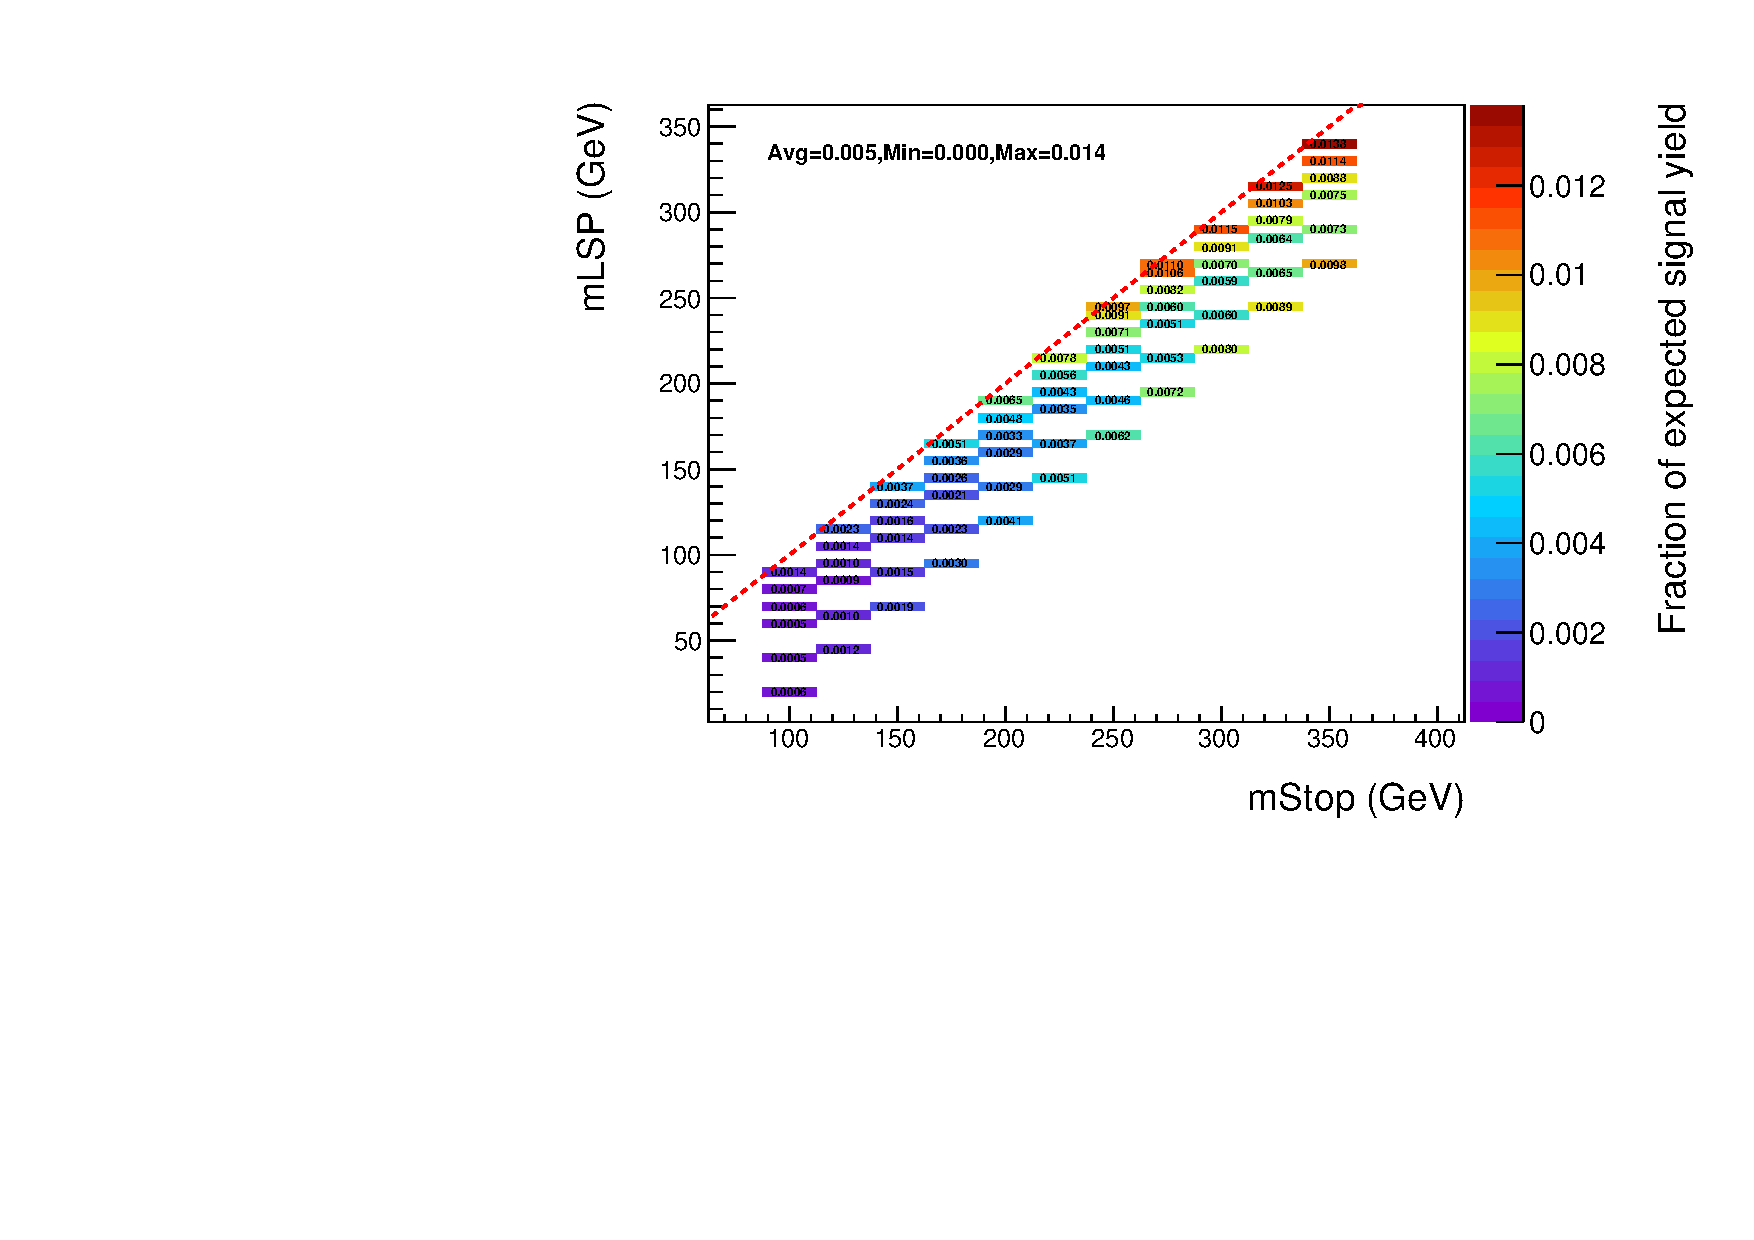
\includegraphics[width=\textwidth]{Figs/sms/t2cc/v37/effs/T2cc_had_eff_maps_eq0b_le3j_SITV.pdf}
    \caption{Signal region, (2--3,0)}
    \label{fig:t2cc_sig_eff_le3j_0b}
  \end{subfigure}
  \begin{subfigure}[b]{0.47\textwidth}
    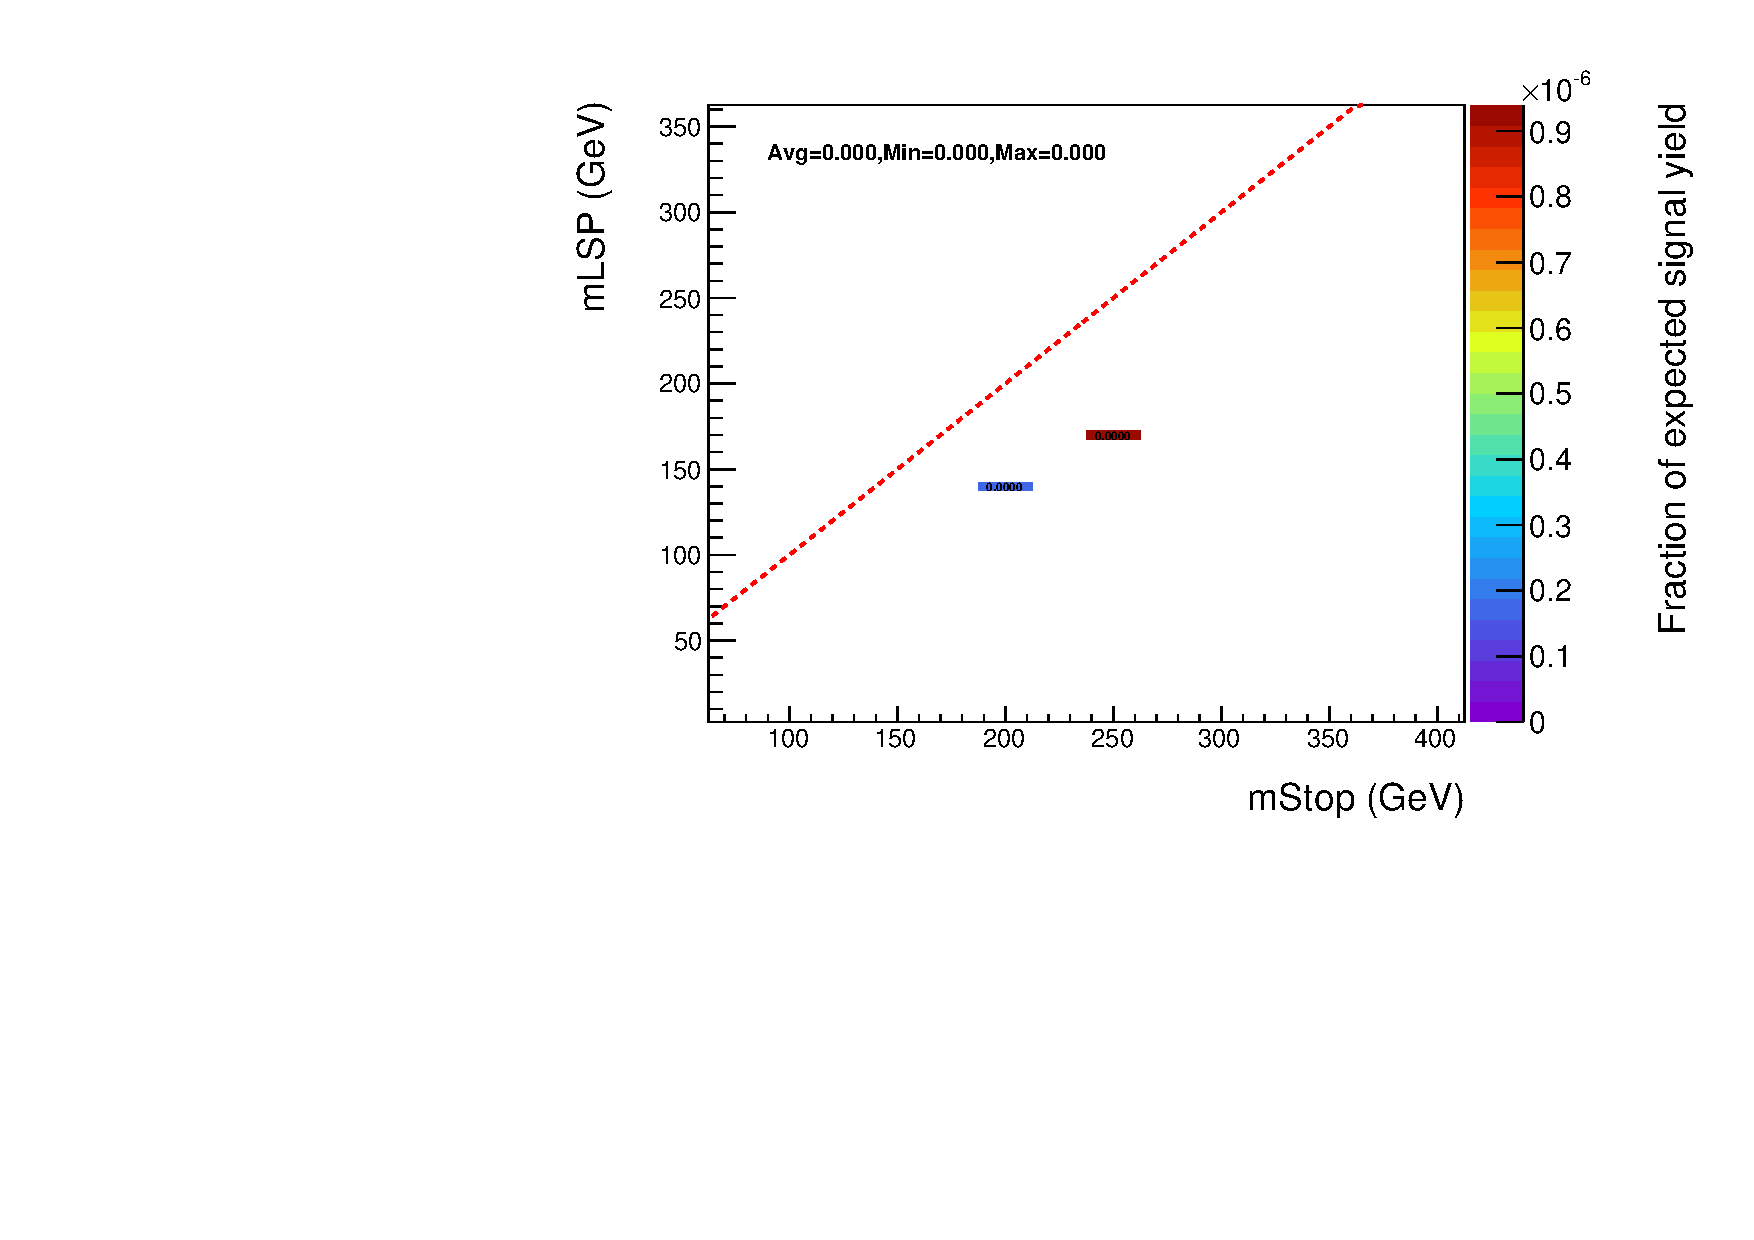
\includegraphics[width=\textwidth]{Figs/sms/t2cc/v37/effs/T2cc_muon_eff_maps_eq0b_le3j_SITV.pdf}
    \caption{\mj region, (2--3,0)}
    \label{fig:t2cc_mu_eff_le3j_0b}
  \end{subfigure} \\
  \begin{subfigure}[b]{0.47\textwidth}
    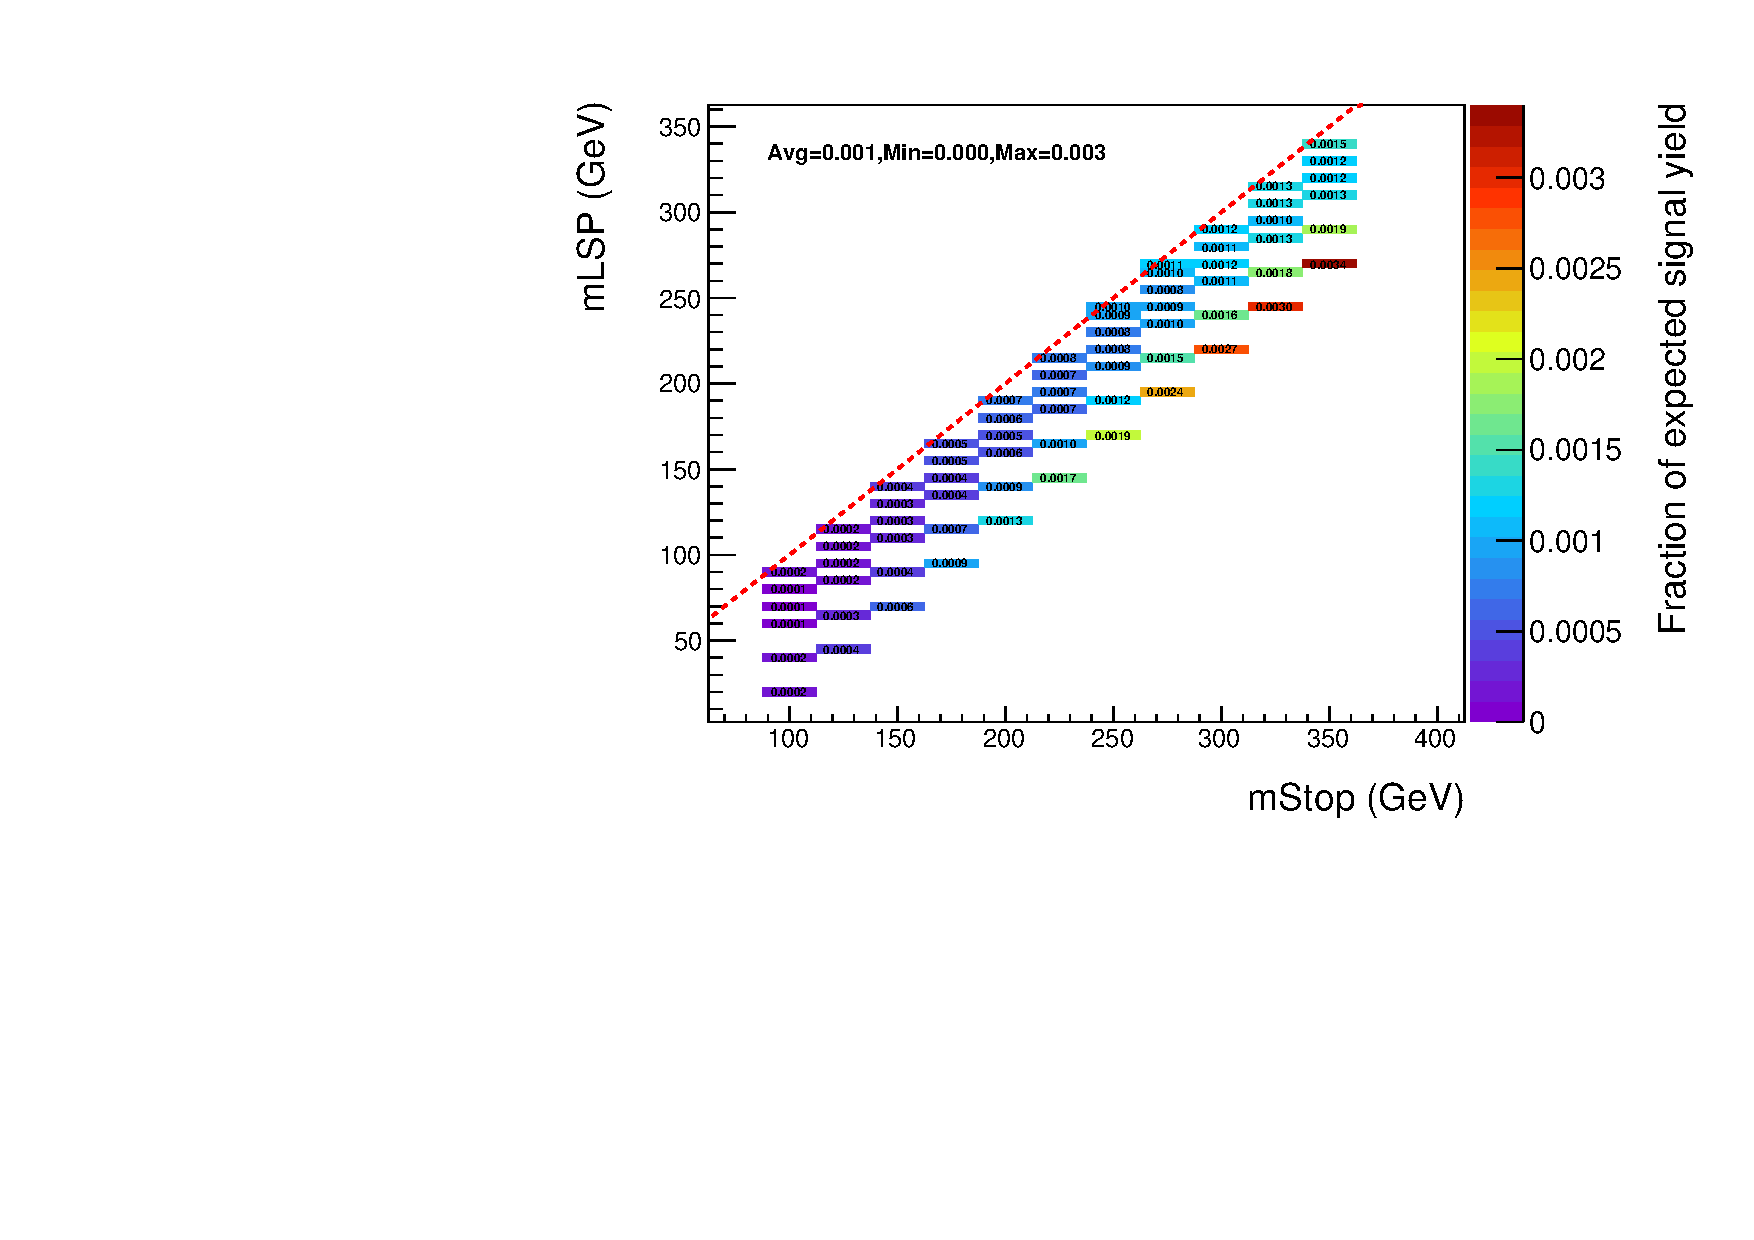
\includegraphics[width=\textwidth]{Figs/sms/t2cc/v37/effs/T2cc_had_eff_maps_eq1b_le3j_SITV.pdf}
    \caption{Signal region, (2--3,1)}
    \label{fig:t2cc_sig_eff_le3j_1b}
  \end{subfigure}
  \begin{subfigure}[b]{0.47\textwidth}
    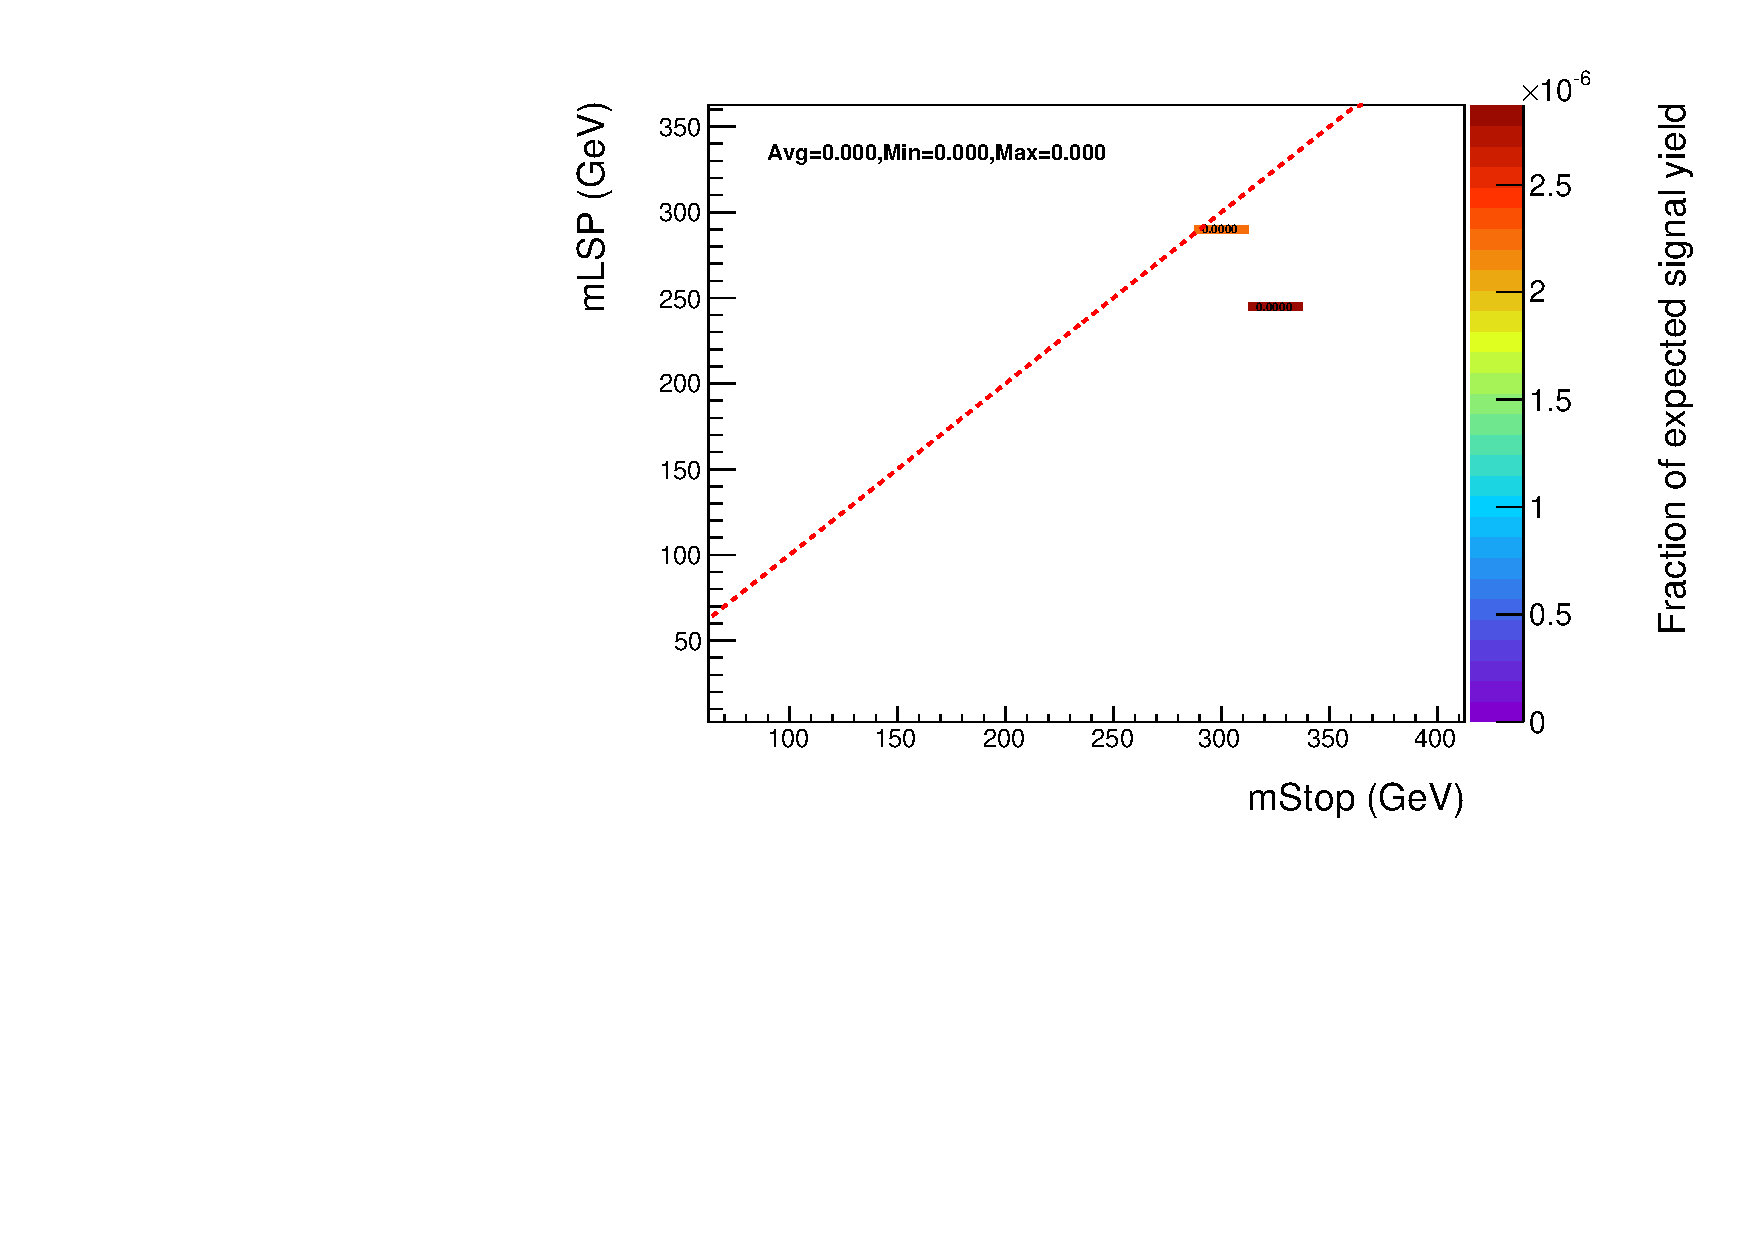
\includegraphics[width=\textwidth]{Figs/sms/t2cc/v37/effs/T2cc_muon_eff_maps_eq1b_le3j_SITV.pdf}
    \caption{\mj region, (2--3,1)}
    \label{fig:t2cc_mu_eff_le3j_1b}
  \end{subfigure} \\
  \begin{subfigure}[b]{0.47\textwidth}
    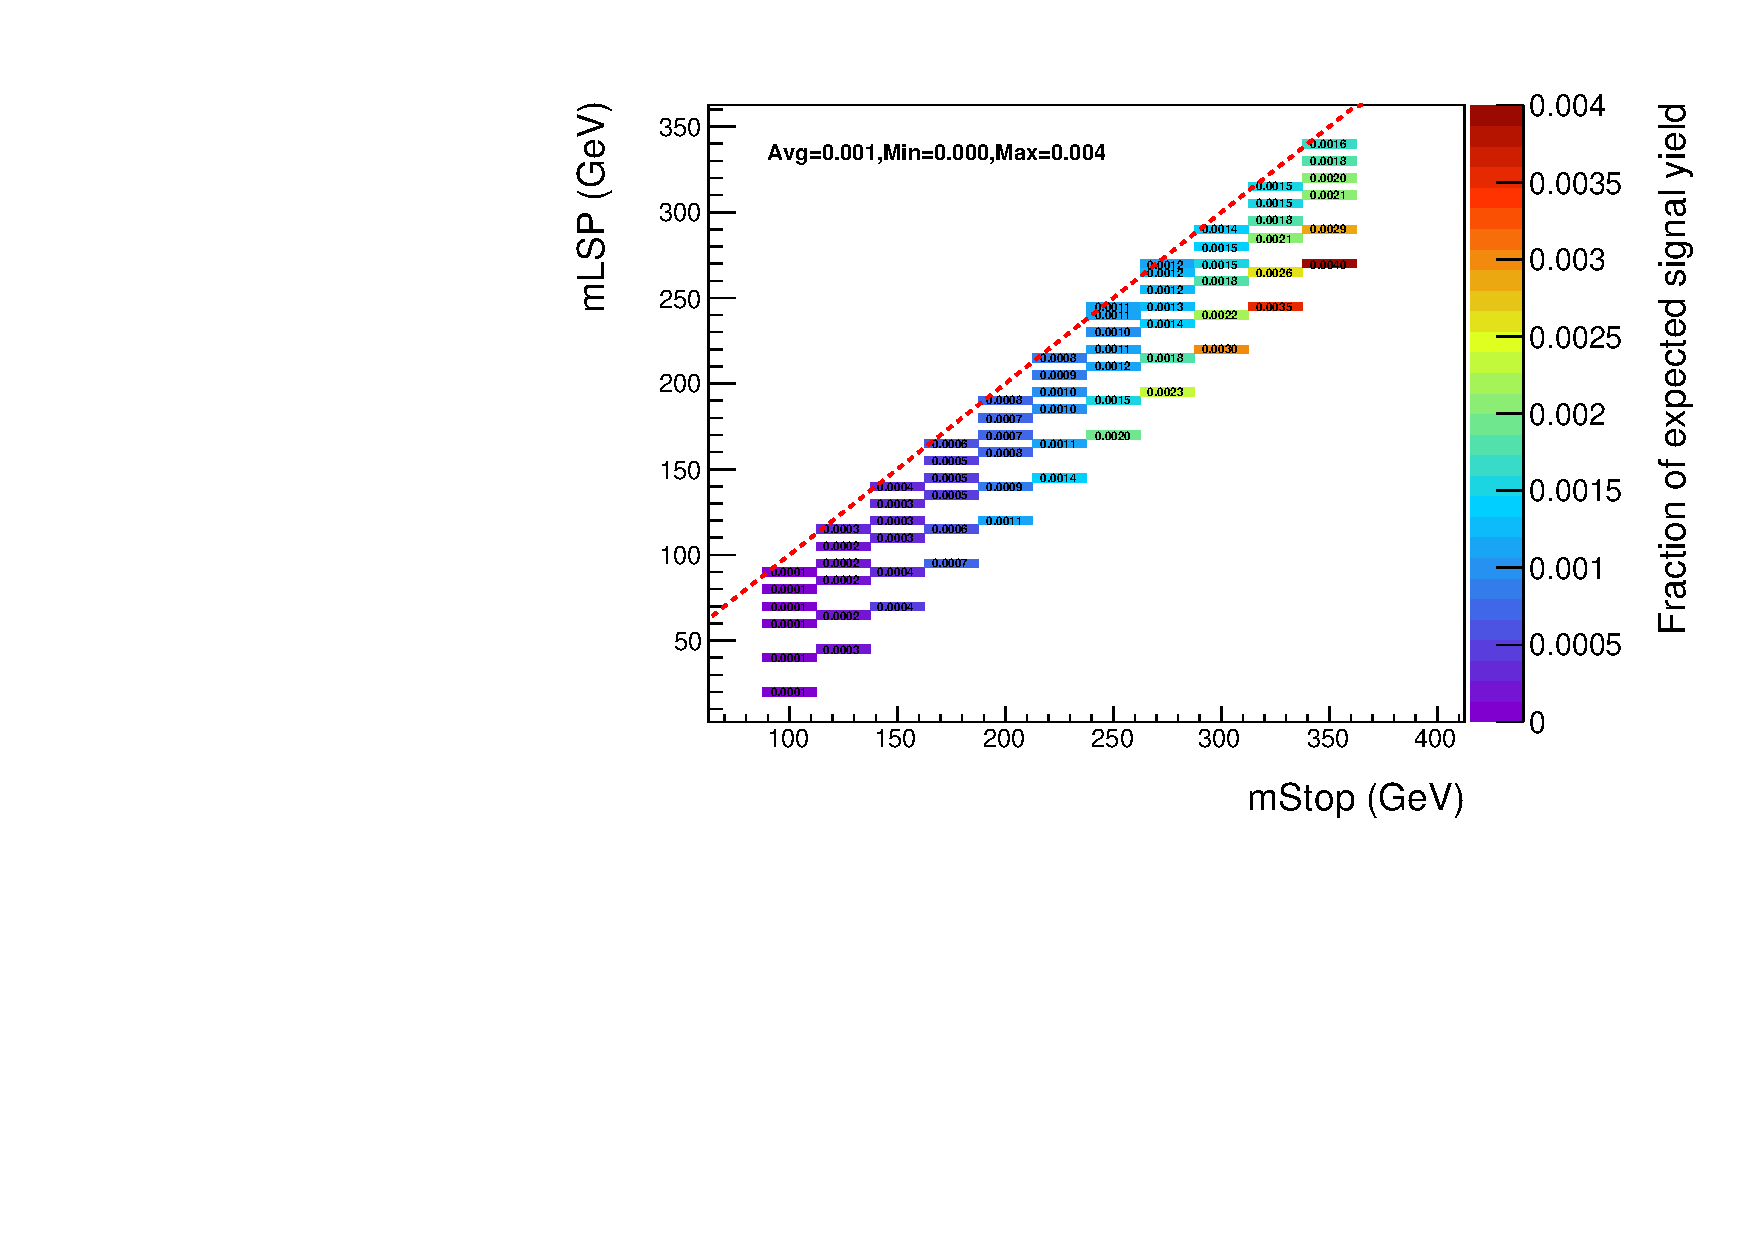
\includegraphics[width=\textwidth]{Figs/sms/t2cc/v37/effs/T2cc_had_eff_maps_eq0b_ge4j_SITV.pdf}
    \caption{Signal region, ($\geq 4$,0)}
    \label{fig:t2cc_sig_eff_ge4j_0b}
  \end{subfigure}
  \begin{subfigure}[b]{0.47\textwidth}
    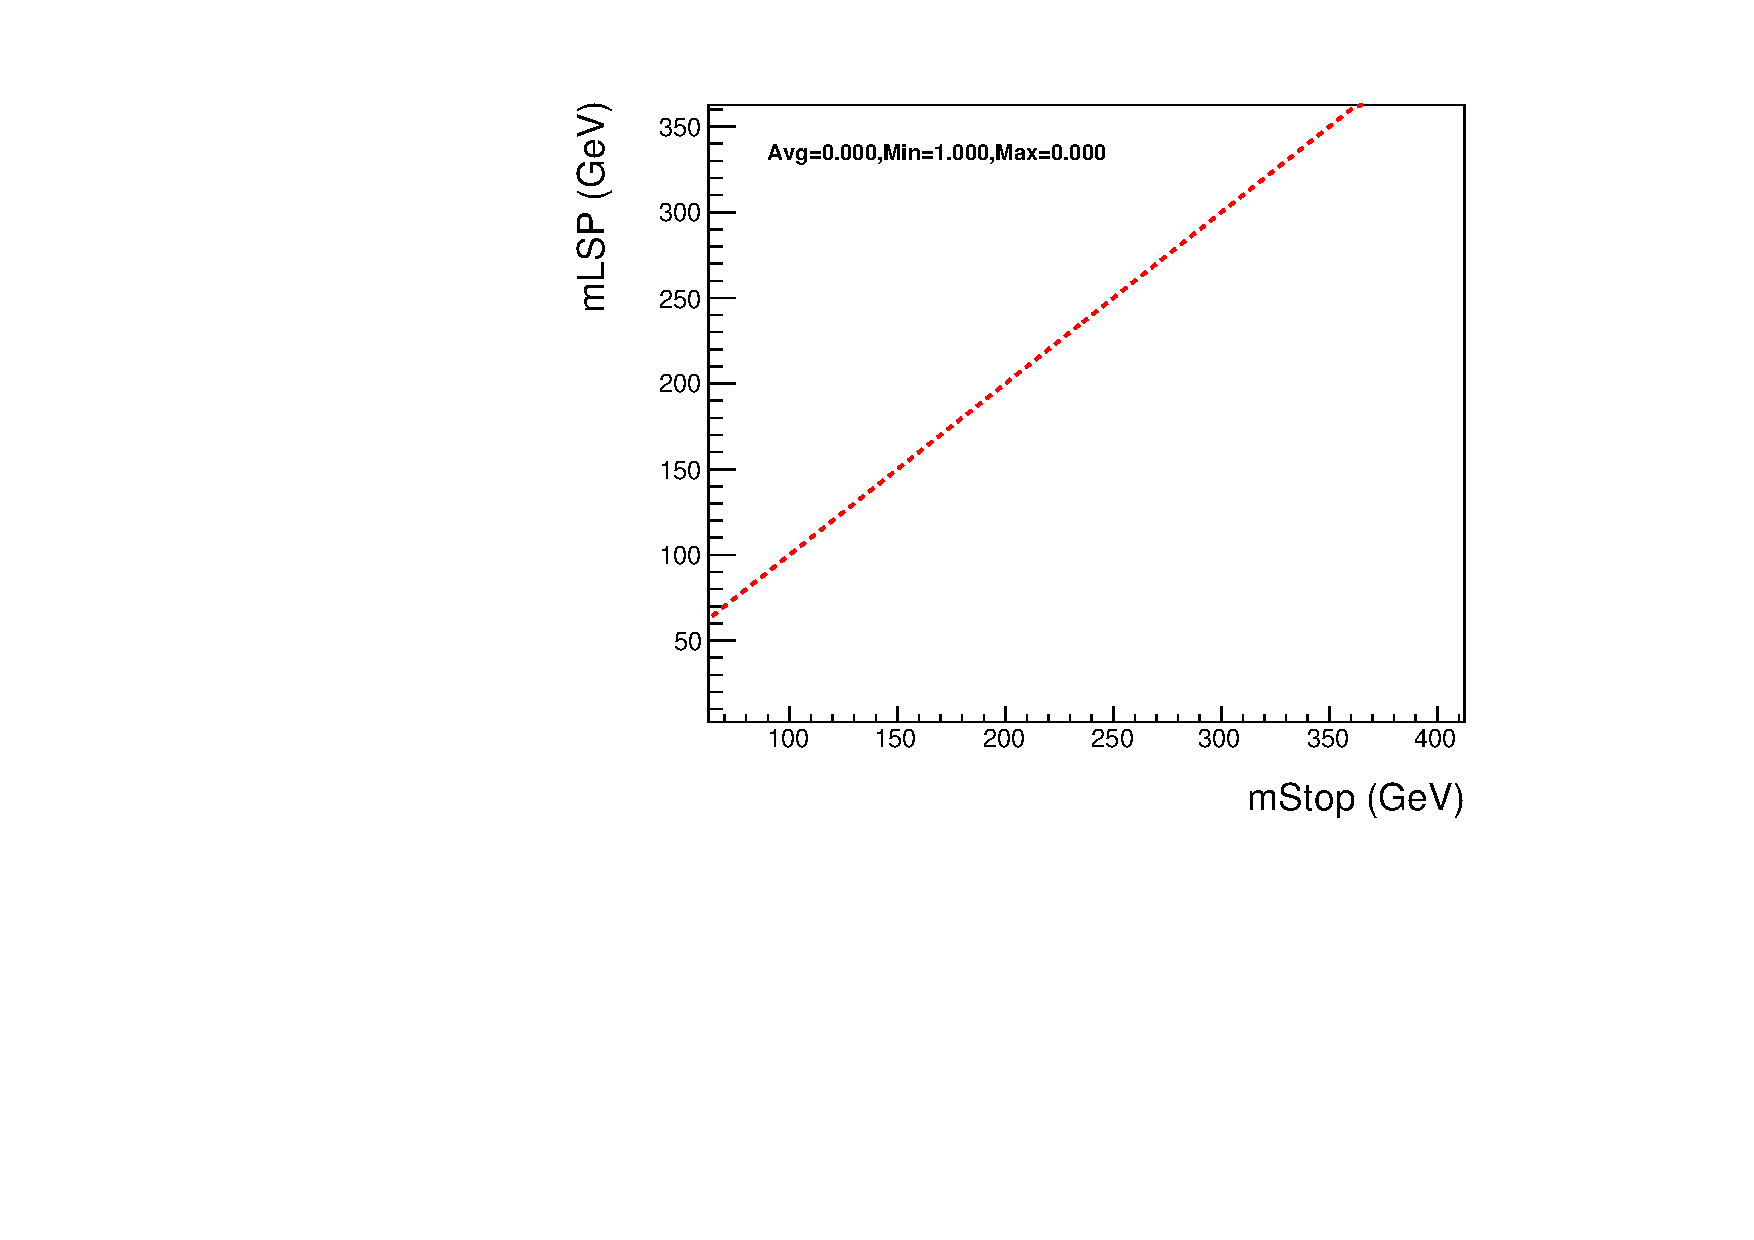
\includegraphics[width=\textwidth]{Figs/sms/t2cc/v37/effs/T2cc_muon_eff_maps_eq0b_ge4j_SITV.pdf}
    \caption{\mj region, ($\geq 4$,0)}
    \label{fig:t2cc_mu_eff_ge4j_0b}
  \end{subfigure} \\
  \begin{subfigure}[b]{0.47\textwidth}
    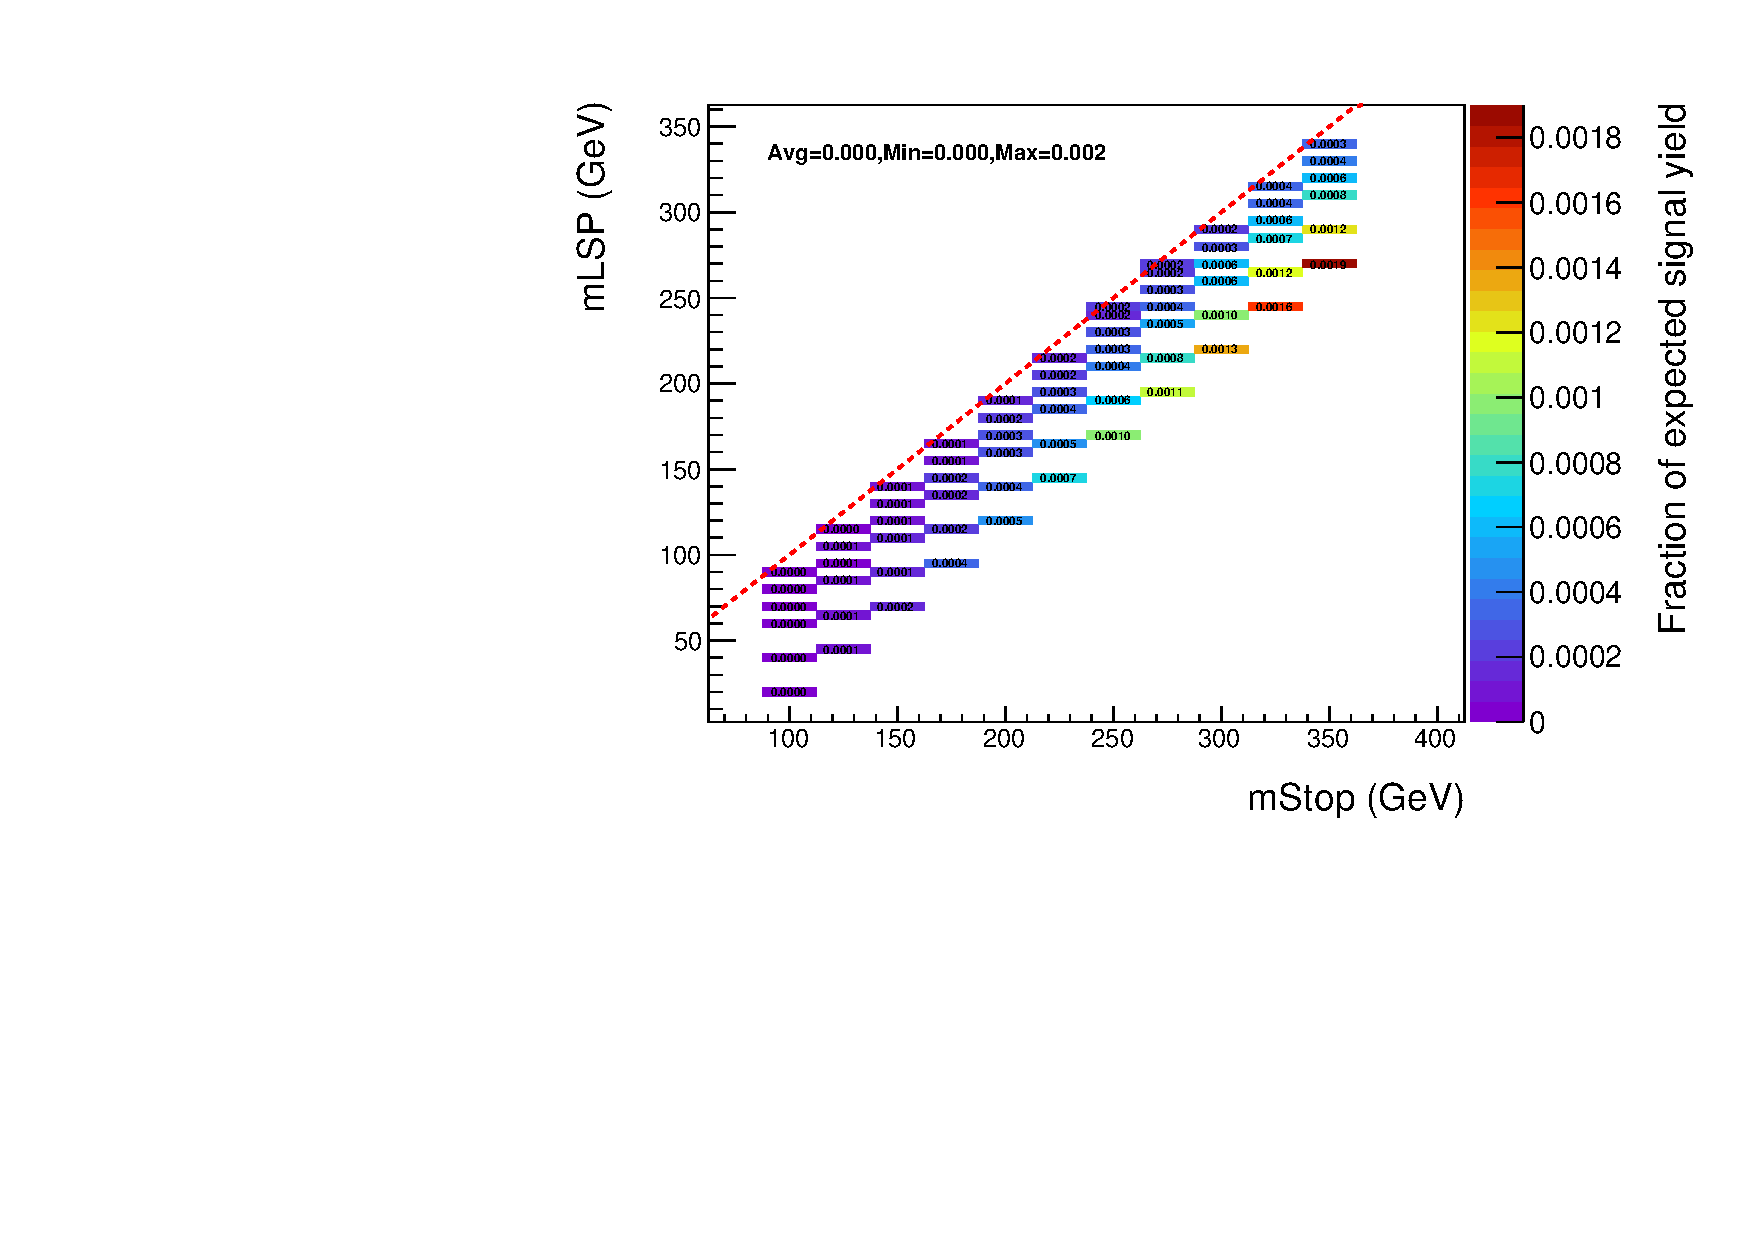
\includegraphics[width=\textwidth]{Figs/sms/t2cc/v37/effs/T2cc_had_eff_maps_eq1b_ge4j_SITV.pdf}
    \caption{Signal region, ($\geq 4$,1)}
    \label{fig:t2cc_sig_eff_ge4j_1b}
  \end{subfigure}
  \begin{subfigure}[b]{0.47\textwidth}
    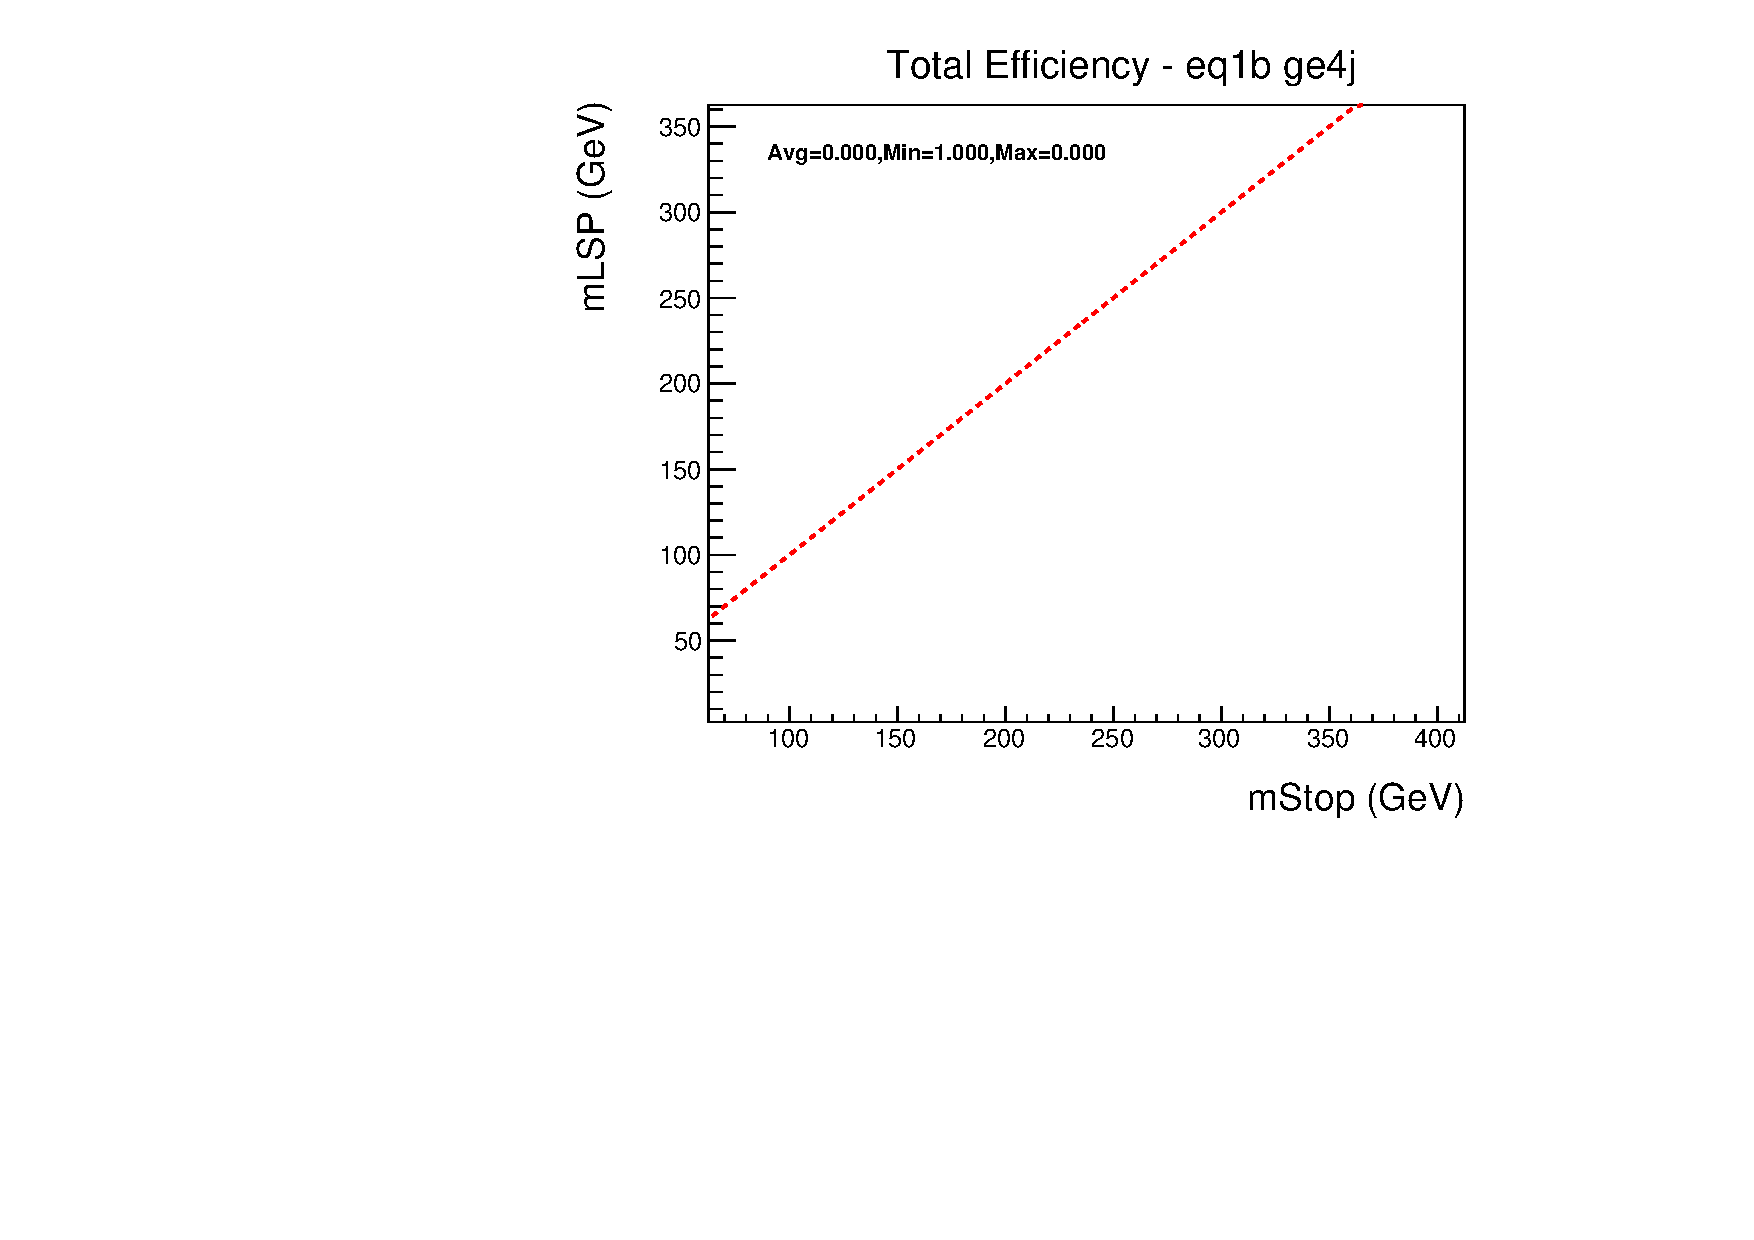
\includegraphics[width=\textwidth]{Figs/sms/t2cc/v37/effs/T2cc_muon_eff_maps_eq1b_ge4j_SITV.pdf}
    \caption{\mj region, ($\geq 4$,1)}
    \label{fig:t2cc_mu_eff_ge4j_1b}
  \end{subfigure} \\
  \caption{Signal efficiency times acceptance for the \Ttwocc simplified, for 
  the hadronic selection (left) and the \mj selection (right), shown for the 
  four most sensitive analysis categories with an inclusive selection on \HT.}
  \label{fig:t2cc_eff}
\end{figure}

% \begin{figure}[h!]
%   \centering
%   \begin{subfigure}[b]{0.6\textwidth}
%     \includegraphics[width=\textwidth, trim=0 0 0 30, clip=true]{Figs/sms/t2cc/v24/T2cc_v24_sig_inj_250_170.pdf}
%     \caption{$m_{\sTop} = 250\gev, m_{\rm LSP} = 170\gev$}
%     \label{fig:t2cc_sig_inj_dm80}
%   \end{subfigure}
%   \begin{subfigure}[b]{0.6\textwidth}
%     \includegraphics[width=\textwidth, trim=0 0 0 30, clip=true]{Figs/sms/t2cc/v24/T2cc_v24_sig_inj_250_240.pdf}
%     \caption{$m_{\sTop} = 250\gev, m_{\rm LSP} = 240\gev$}
%     \label{fig:t2cc_sig_inj_dm10}
%   \end{subfigure}
%   \caption{balls}
%   \label{fig:}
% \end{figure}

\begin{table}[ht!]
  \caption{Cutflow table for two mass points ($m_{\sTop} = 250$ \gev, $m_
  {\chiz}=240$ \gev and $m_{\sTop} = 250$ \gev, $m_{\chiz}=170$ \gev) of the
  \texttt{T2cc} signal model.} \label{tab:t2cc_cutflow}
  \centering
  \footnotesize
  \begin{tabular}{ lcc }
    \hline
    \hline
    Cut Name    & \multicolumn{2}{c}{Cumlative Eff. (\%)}\\
    \hline
    ($m_{\sTop}$, $m_{\chiz}$)& (250, 240) & (250, 170) \\
    \hline
  Event Counter & 100.00 & 100.00 \\
  $\nj \geq 2$  & 12.99 & 59.52 \\
  MET Filters & 12.99  & 59.52 \\
  Vertex Noise Filter & 12.99 & 59.52 \\
  HBHE Noise Filter & 12.99 & 59.52 \\
  DeadECAL Filter & 10.77 & 43.88\\
  $n_{e} = 0$ & 10.77 & 43.88\\
  $n_{\gamma} = 0$  & 10.77 & 43.7\\
  $n_{\mu} = 0$ & 10.77 & 43.7\\
  $\text{EMF}_{max}$ for all jets > 0.1 & 10.77 & 43.7 \\
  Leading jet \Pt > 100 \gev  & 7.37 & 24.79\\
  Leading jet $\eta$ < 2.5  & 7.04 & 24.21\\
  Sub-Leading jet \Pt > 100 \gev  & 2.31 & 8.92 \\
  $n_{j, fail} = 0$ & 2.26 & 8.66\\
  $\Delta R(\mu^i_{fail}, jet^j) < 0.5$ & 2.26 & 8.65\\
  $(\sum_{}^{n_{vertices}}{\Pt}$) / \HT & 2.26 & 8.65\\
  recHitCut & 2.26 & 8.65\\
  $n_{SIT} = 0$ & 2.09 & 8.03\\
  \mindphistar > 0.3  & 1.84 & 5.42\\
  \mhtmet < 1.25  & 1.68 & 4.46\\
  \HT > 375 \gev  & 0.90 & 2.05\\
  \alphat > 0.55  & 0.45 & 0.40\\
  \mhtmet < 1.25  & 0.45 & 0.40\\
    \hline
    \hline
  \end{tabular}
\end{table}


\subsection{T2\_4body}
\label{sec:t2degen_eff}

The signal efficiency times acceptance distributions for the \texttt{T2degen} model,
\Ttwodegen, are shown 
in figure~\ref{fig:t2_4body_eff} in the four most sensitive analysis categories,
with an inclusive \HT selection, both for the hadronic and \mj selections. There
are strong similarities with those shown earlier for the \texttt{T2cc} model, 
both in magnitude and distribution about the plane. At small values of \deltam, 
given that the entire SUSY decay system becomes invisible due to a lack of 
kinematic phase space, both models show very similar efficiencies, where 
acceptance is almost entirely due to hard ISR jets within acceptance. There is a
significant difference however, when a b-tagged jet is required, for example in 
the \njlow, \nb= 1 category (figure~\ref{fig:t2_4body_sig_eff_le3j_1b}), where
the presence of a jet originating from a real 
b quark improves acceptance, particularly away from the diagonal where this jet 
would be more likely to pass analysis thresholds. Less significant are the 
efficiencies seen in the \njhigh categories, given the larger number of final 
state objects, each requiring a share of the energy originating from the mass 
splitting of the mother and daughter sparticles.

Also of note is the increase in signal contamination observed in the \mj 
selection, due to the presence of $f\bar{f}$ in the decay chain, potentially 
providing leptons in the final state.

Example cutflows are shown in table~\ref{tab:t2_4body_cutflow} for a mass point
with the smallest mass splitting, at an $m_{\sTop}$ value near the limit of
sensitivity.

% should be v16!!
\begin{figure}[ht!]
  \centering
  \begin{subfigure}[b]{0.47\textwidth}
    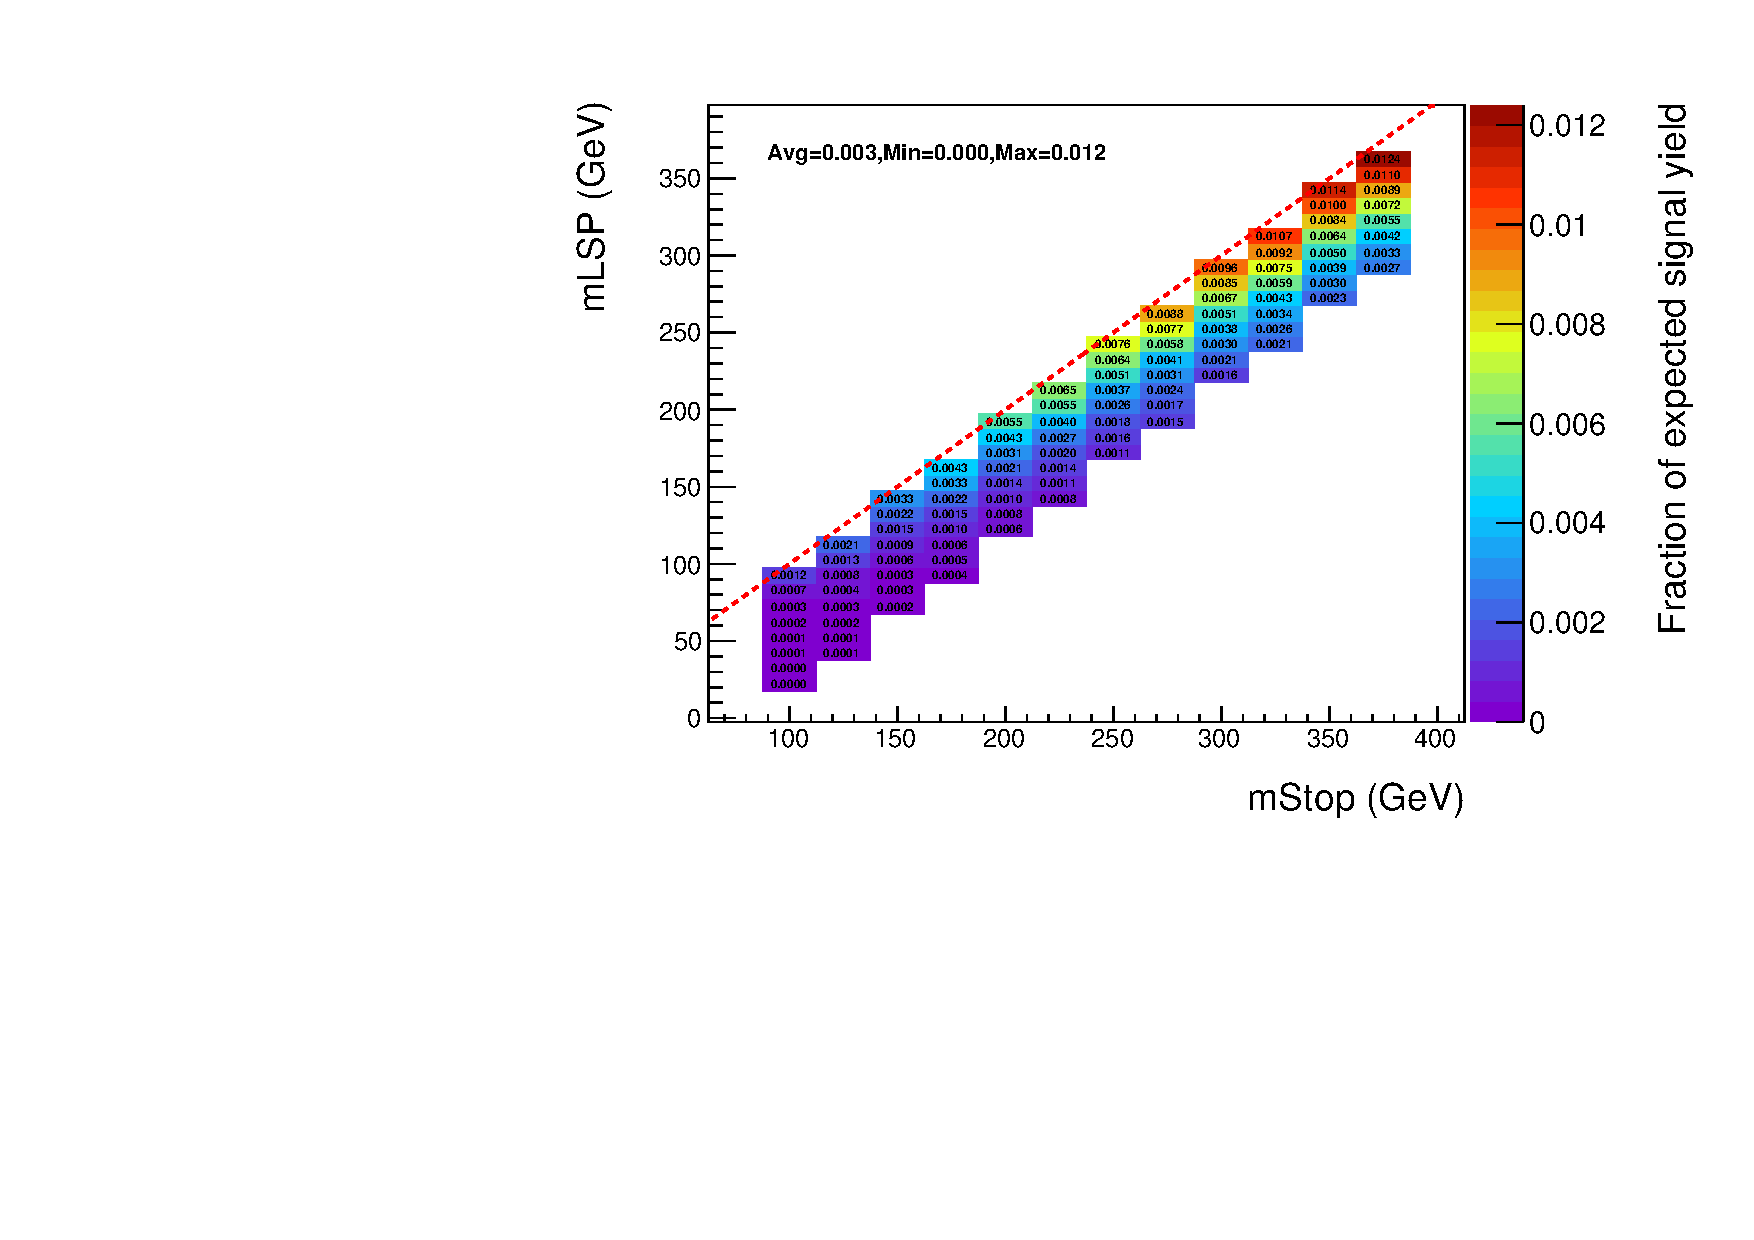
\includegraphics[width=\textwidth]{Figs/sms/t2degen/v23/effs/T2_4body_had_eff_maps_eq0b_le3j_SITV.pdf}
    \caption{Signal region, (2--3,0)}
    \label{fig:t2_4body_sig_eff_le3j_0b}
  \end{subfigure}
  \begin{subfigure}[b]{0.47\textwidth}
    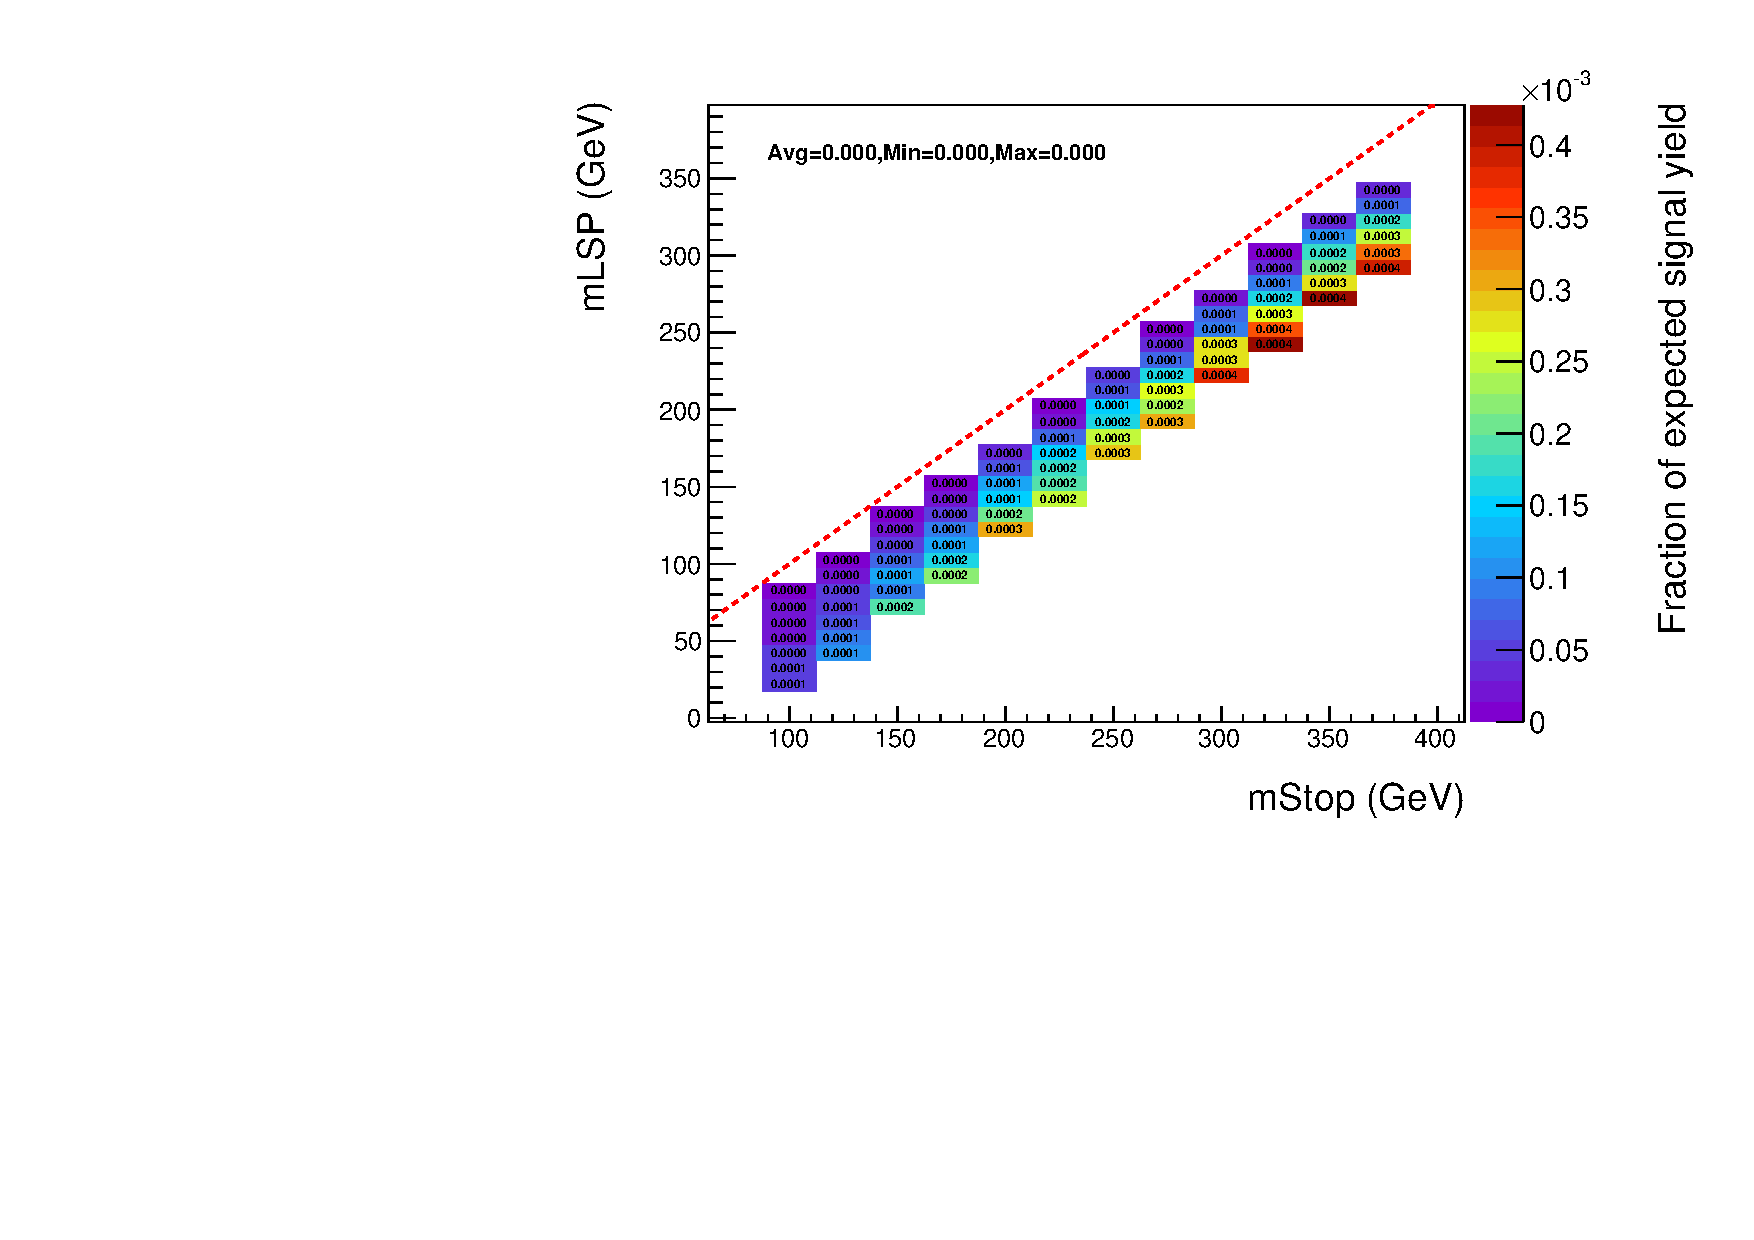
\includegraphics[width=\textwidth]{Figs/sms/t2degen/v23/effs/T2_4body_muon_eff_maps_eq0b_le3j_SITV.pdf}
    \caption{\mj region, (2--3,0)}
    \label{fig:t2_4body_mu_eff_le3j_0b}
  \end{subfigure} \\
  \begin{subfigure}[b]{0.47\textwidth}
    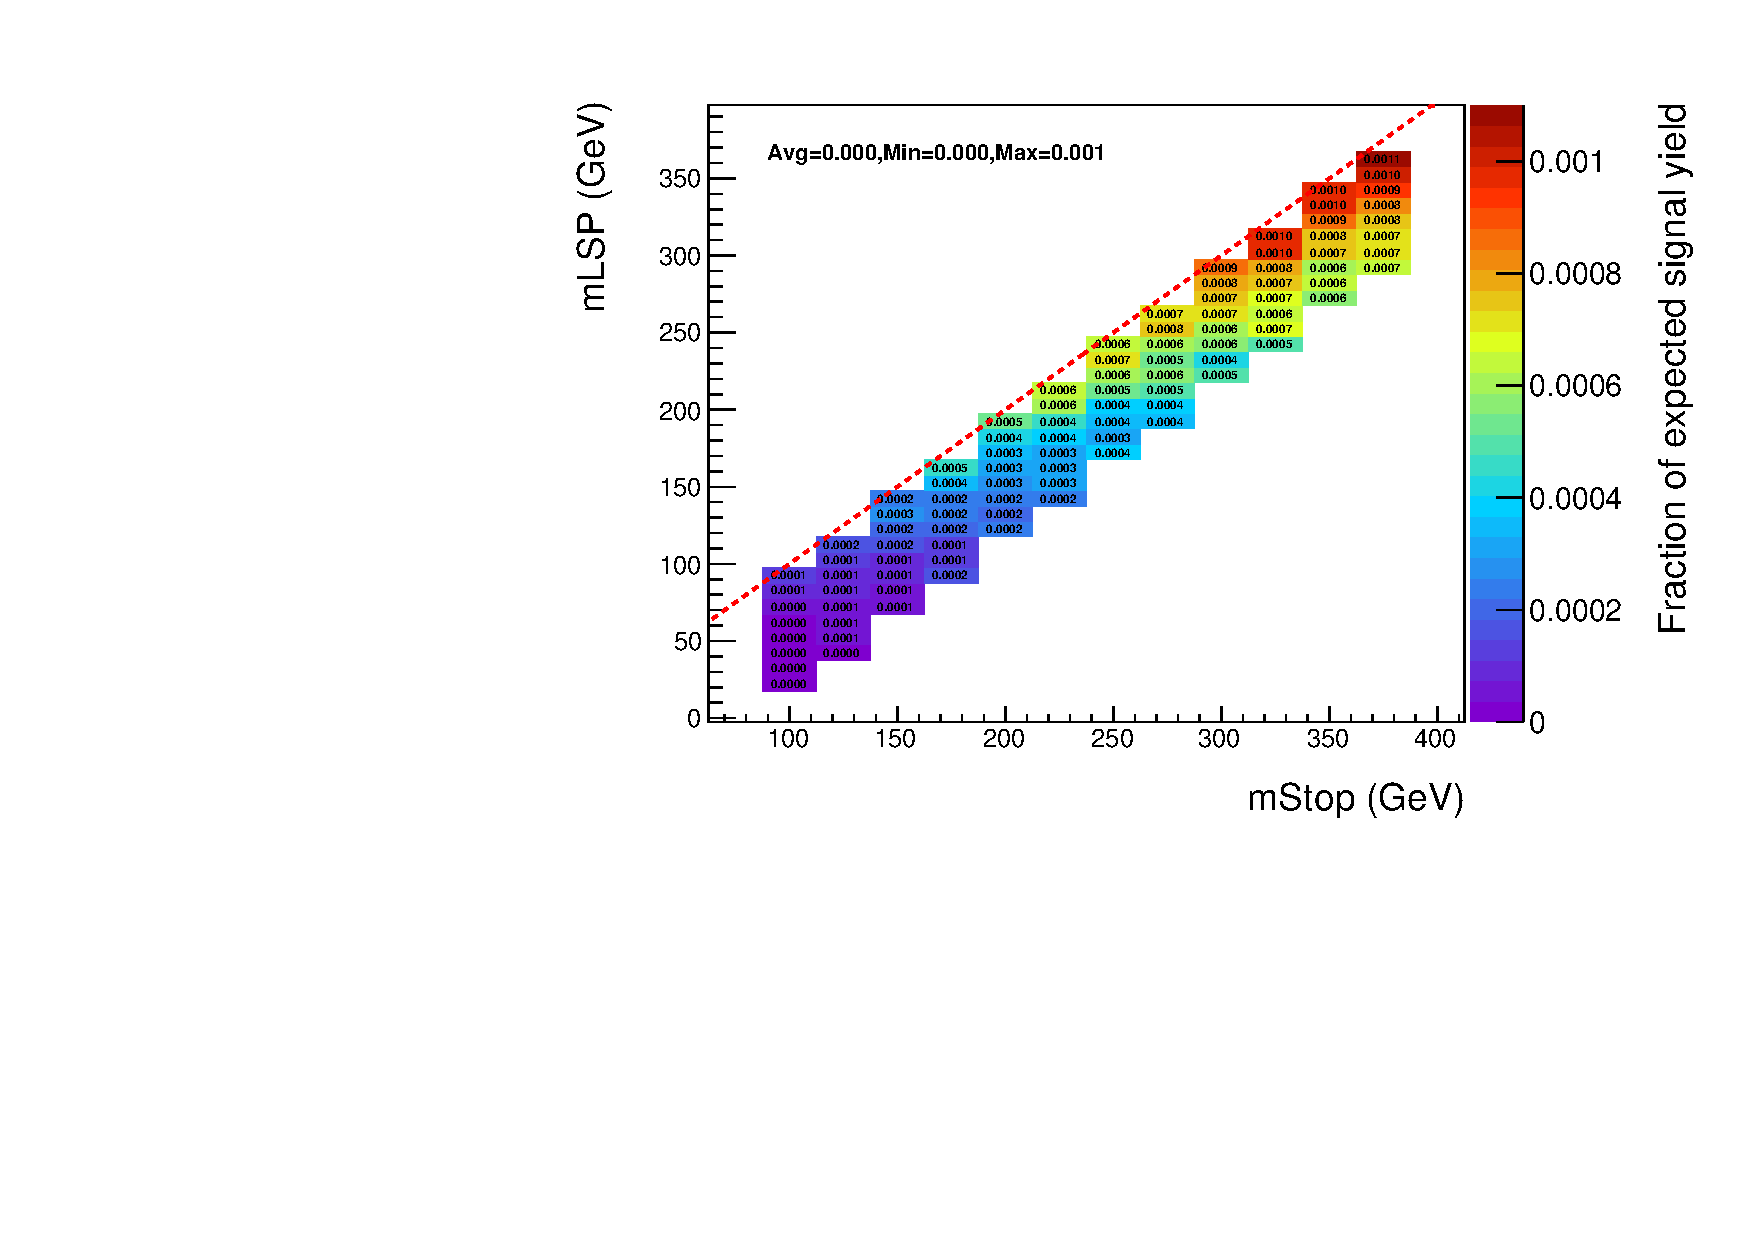
\includegraphics[width=\textwidth]{Figs/sms/t2degen/v23/effs/T2_4body_had_eff_maps_eq1b_le3j_SITV.pdf}
    \caption{Signal region, (2--3,1)}
    \label{fig:t2_4body_sig_eff_le3j_1b}
  \end{subfigure}
  \begin{subfigure}[b]{0.47\textwidth}
    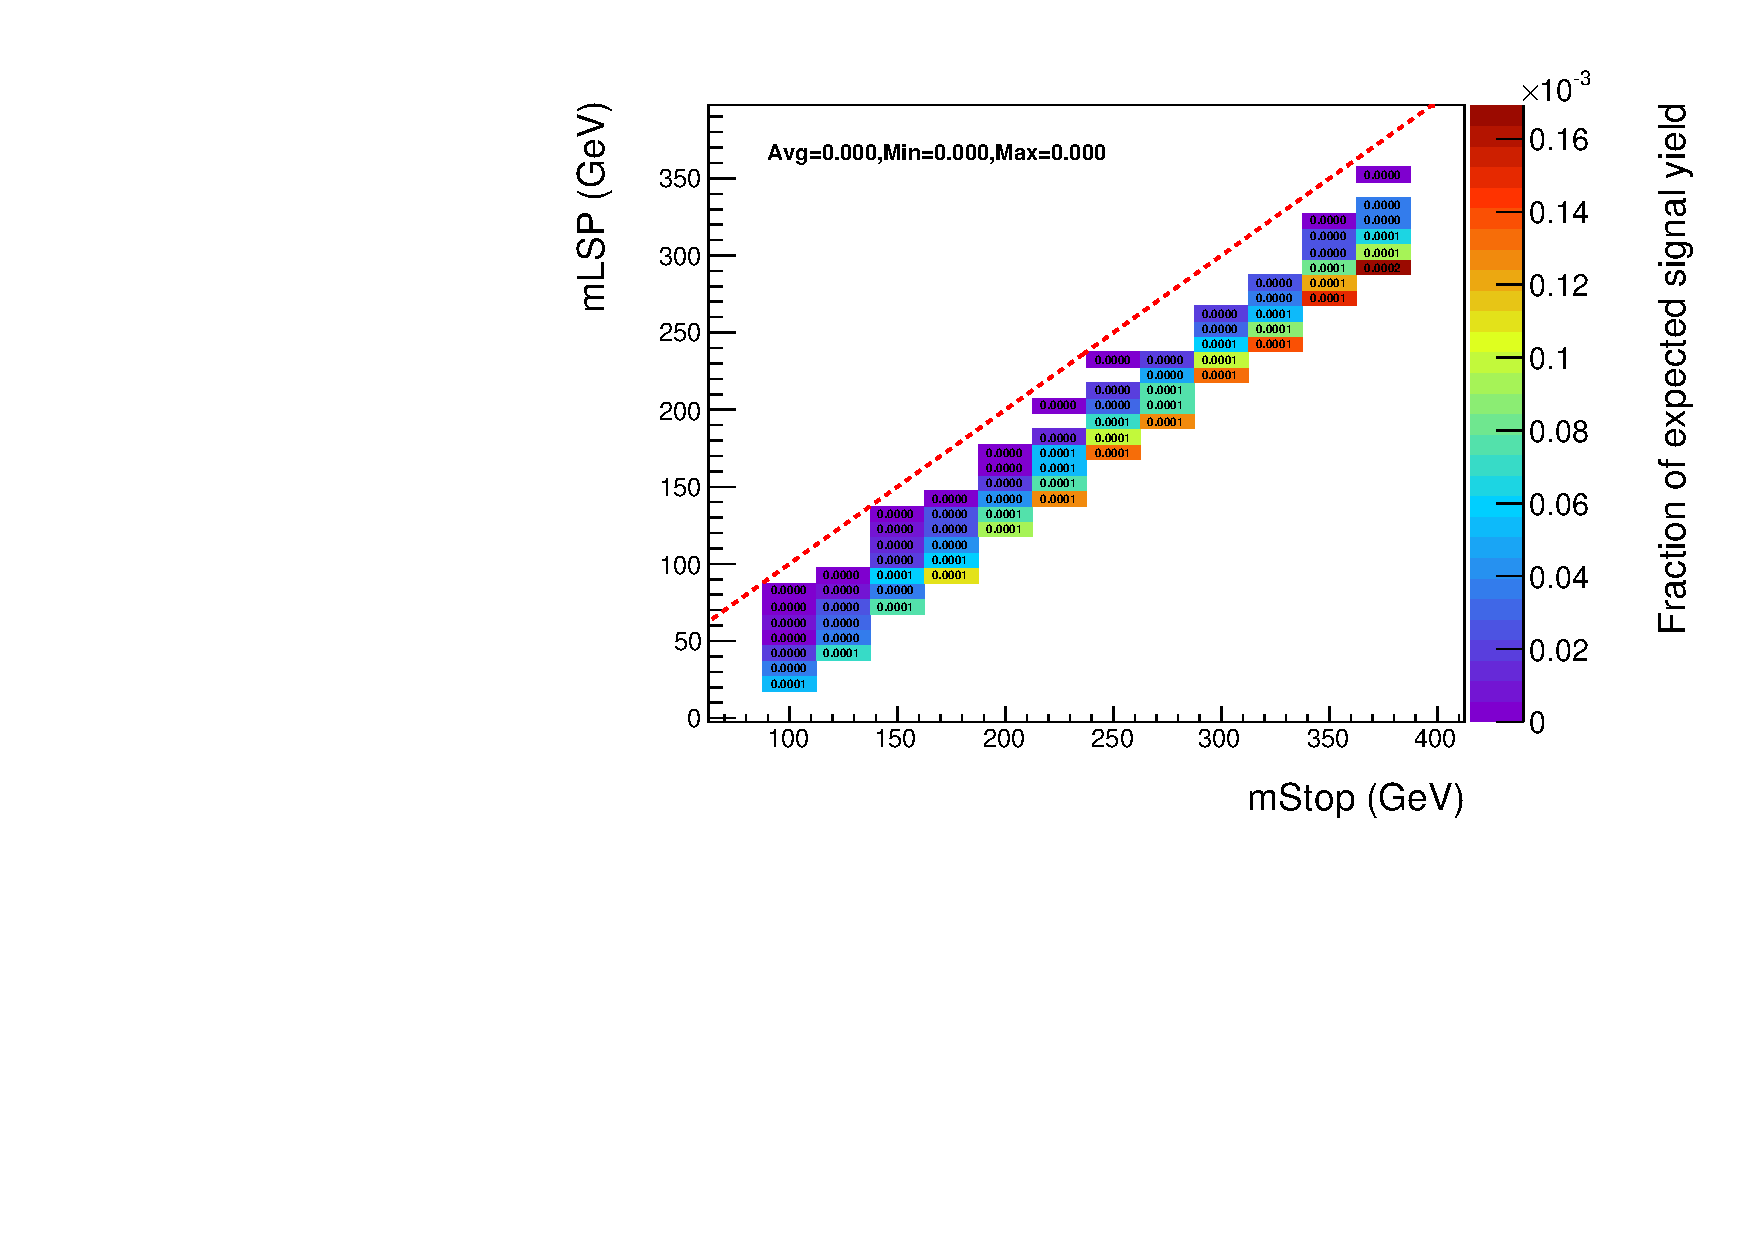
\includegraphics[width=\textwidth]{Figs/sms/t2degen/v23/effs/T2_4body_muon_eff_maps_eq1b_le3j_SITV.pdf}
    \caption{\mj region, (2--3,1)}
    \label{fig:t2_4body_mu_eff_le3j_1b}
  \end{subfigure} \\
  \begin{subfigure}[b]{0.47\textwidth}
    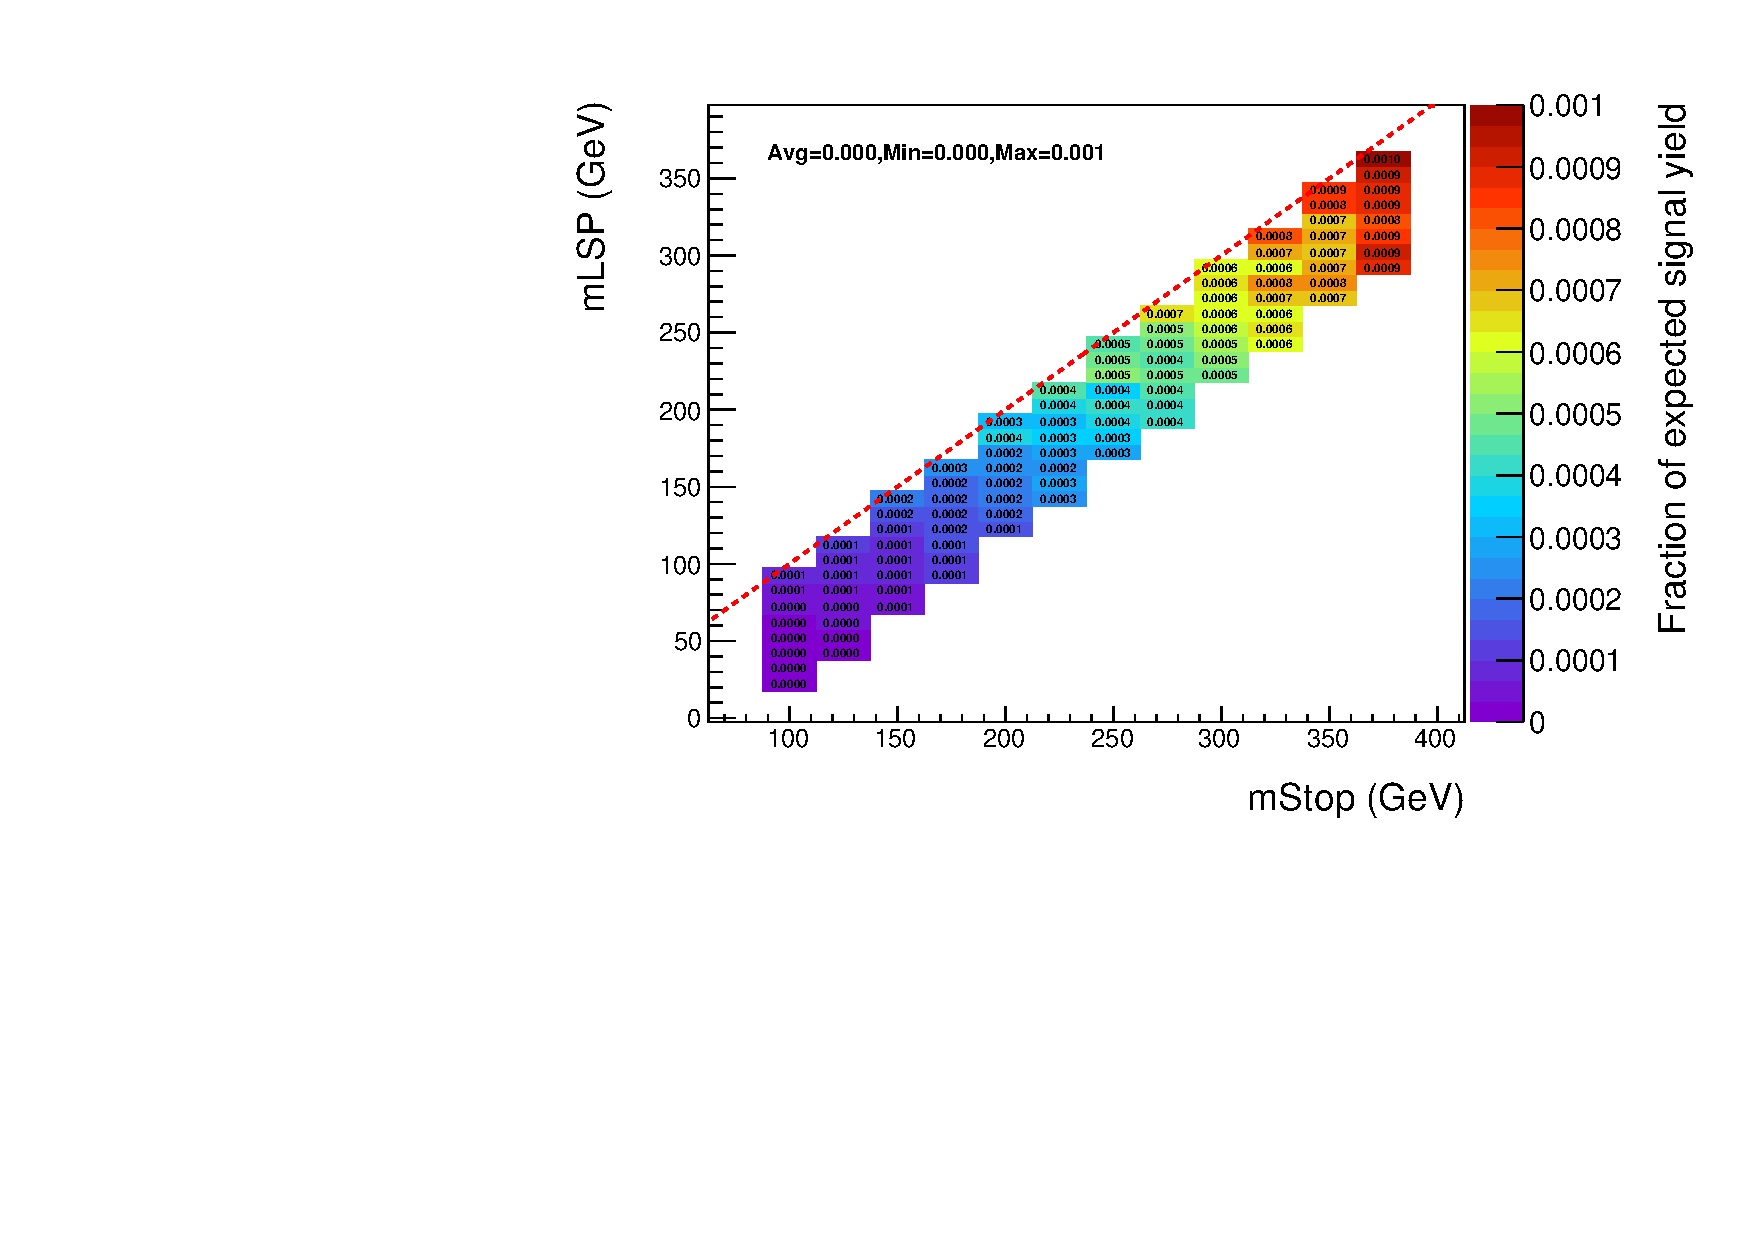
\includegraphics[width=\textwidth]{Figs/sms/t2degen/v23/effs/T2_4body_had_eff_maps_eq0b_ge4j_SITV.pdf}
    \caption{Signal region, ($\geq 4$,0)}
    \label{fig:t2_4body_sig_eff_ge4j_0b}
  \end{subfigure}
  \begin{subfigure}[b]{0.47\textwidth}
    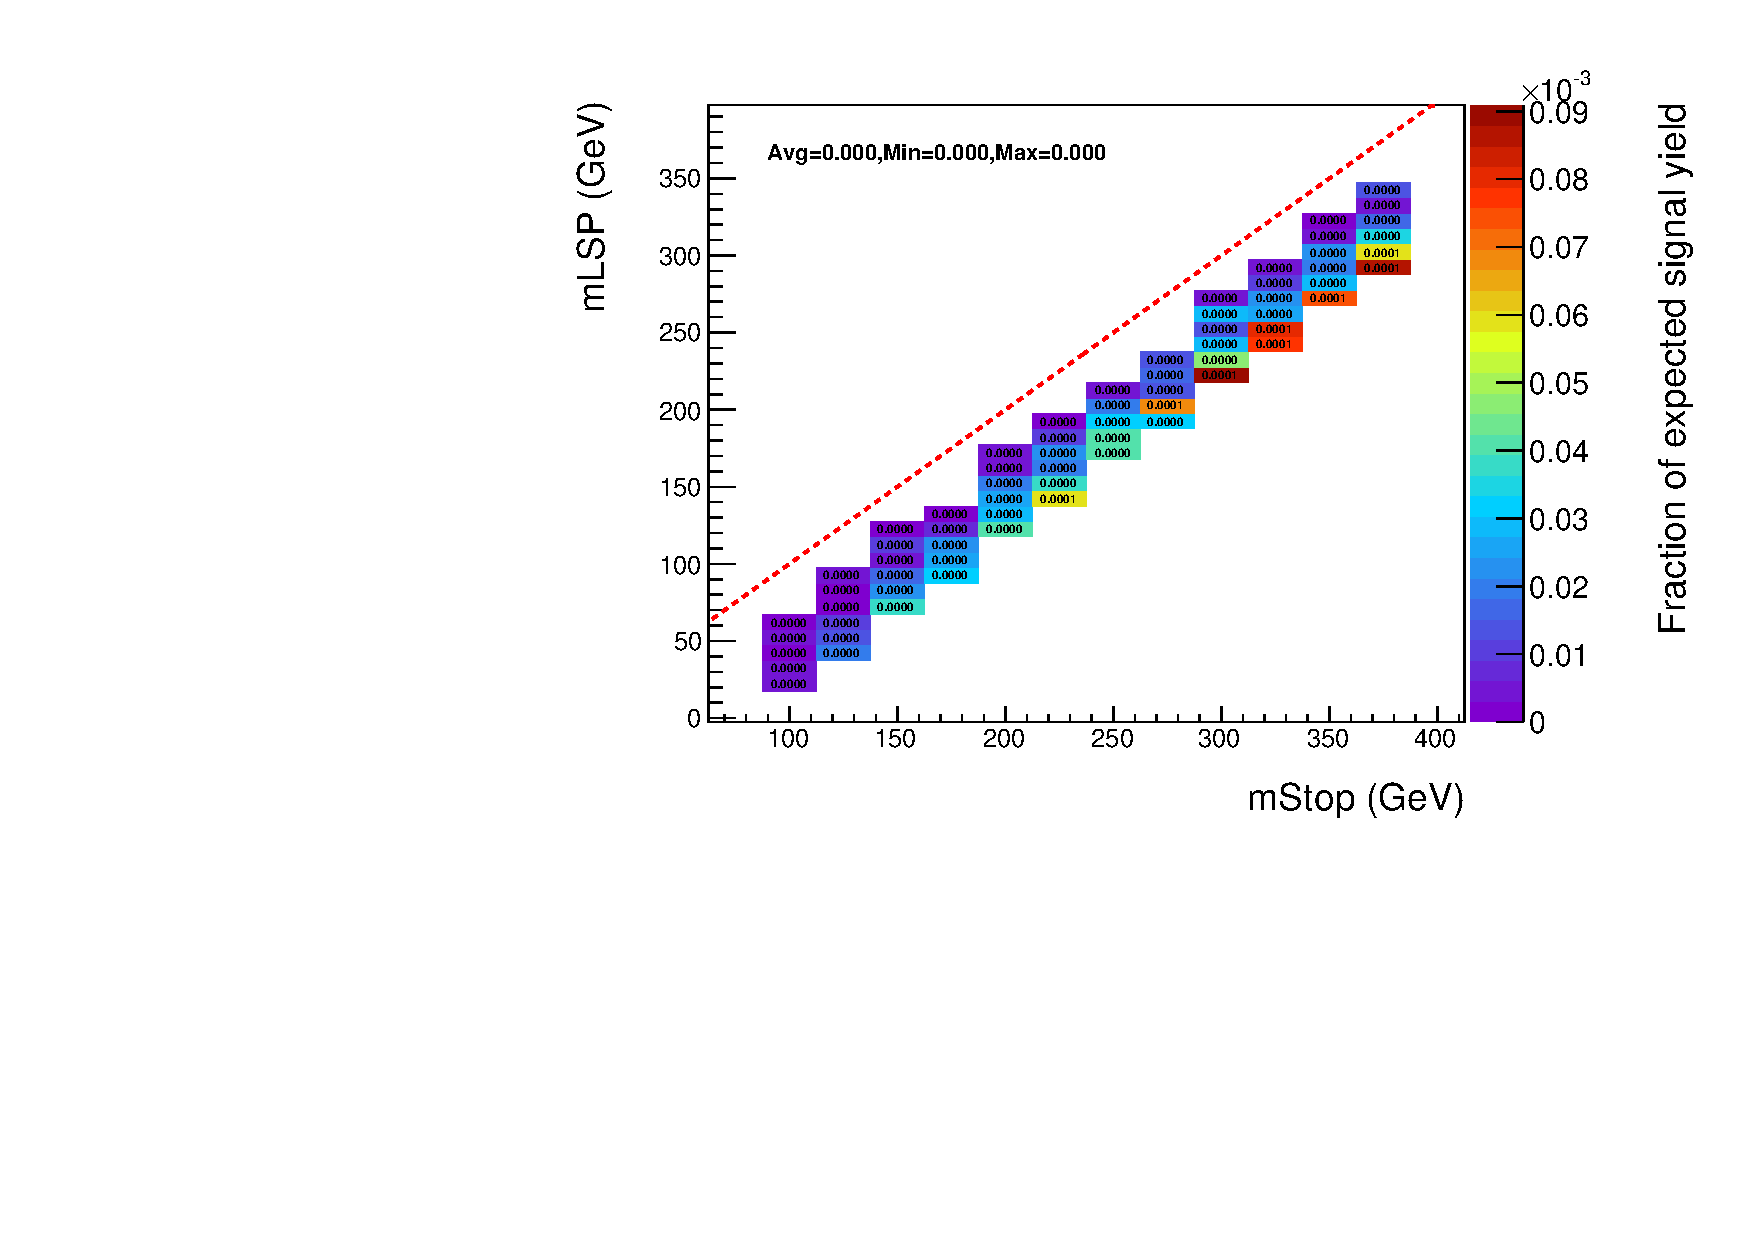
\includegraphics[width=\textwidth]{Figs/sms/t2degen/v23/effs/T2_4body_muon_eff_maps_eq0b_ge4j_SITV.pdf}
    \caption{\mj region, ($\geq 4$,0)}
    \label{fig:t2_4body_mu_eff_ge4j_0b}
  \end{subfigure} \\
  \begin{subfigure}[b]{0.47\textwidth}
    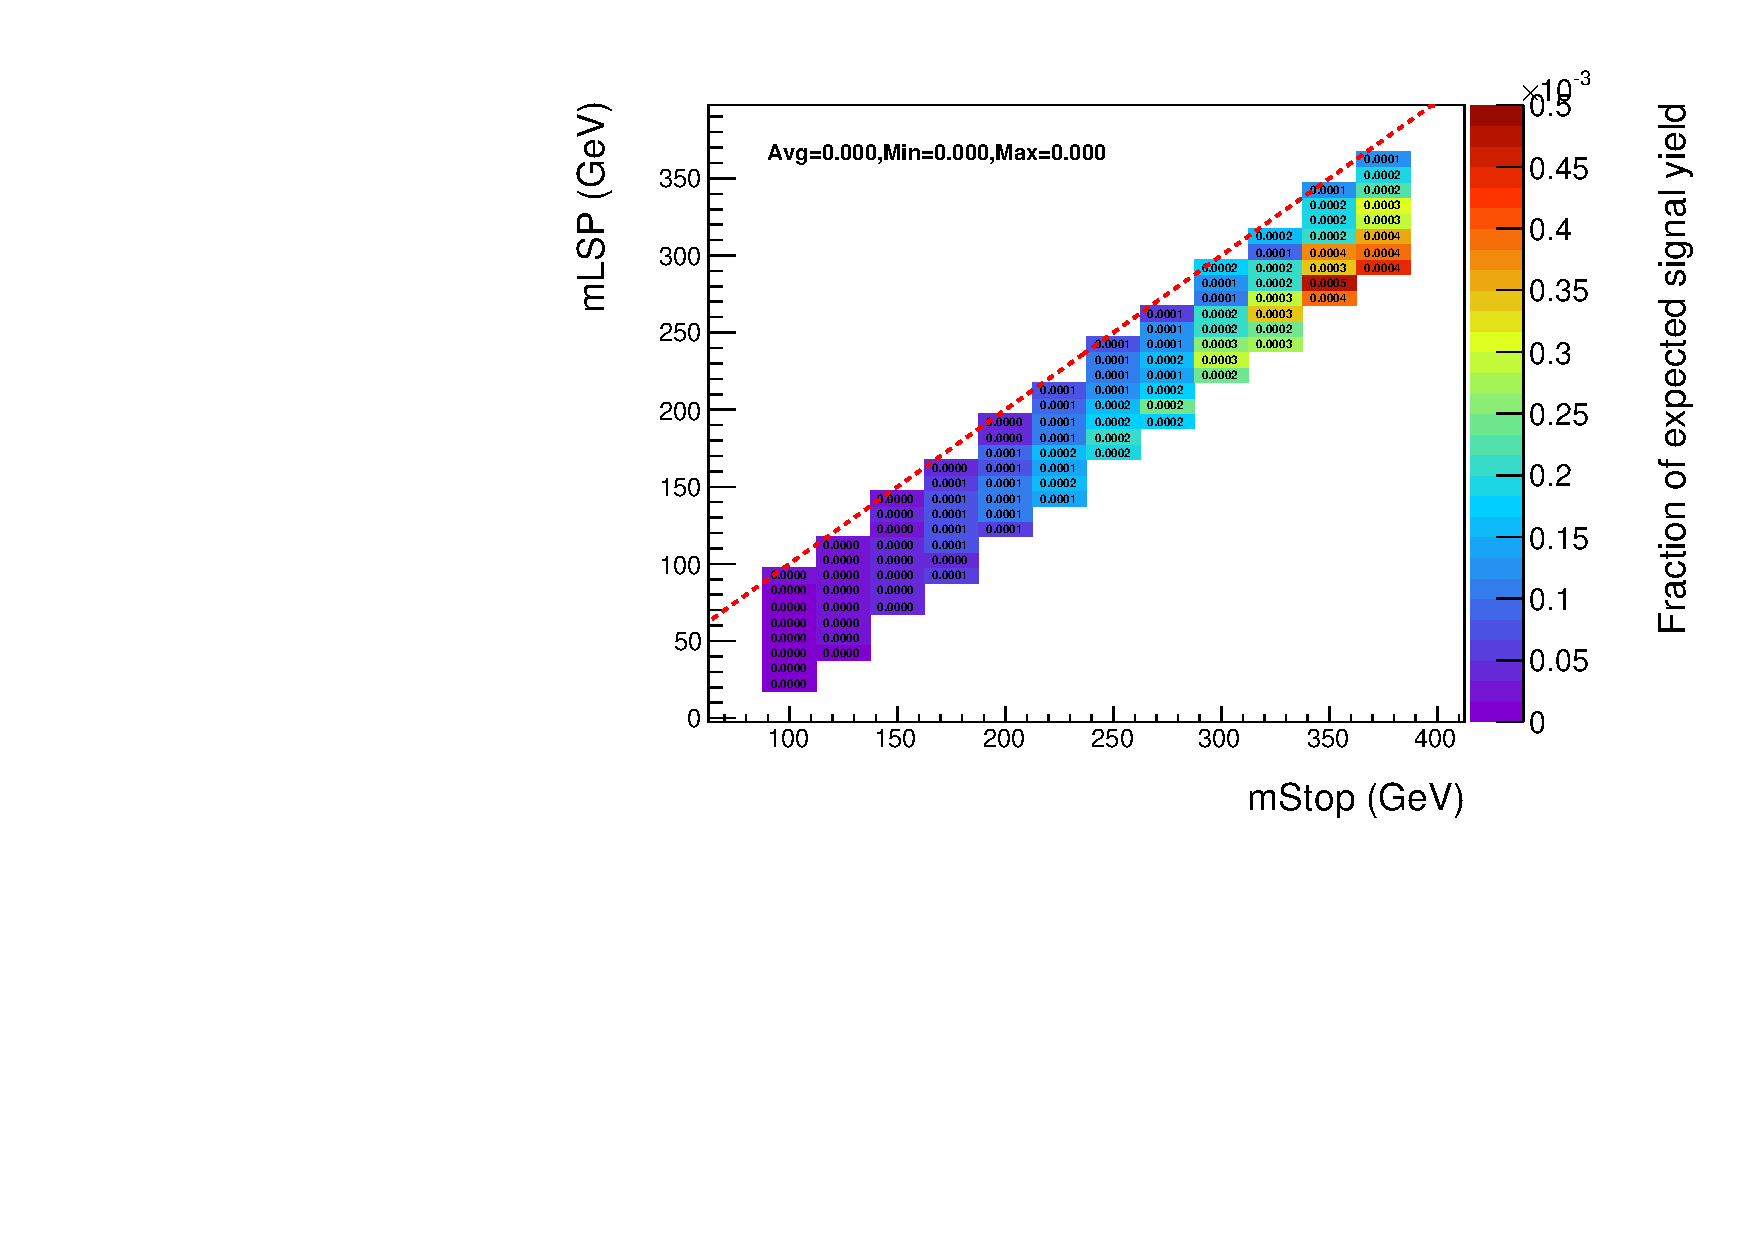
\includegraphics[width=\textwidth]{Figs/sms/t2degen/v23/effs/T2_4body_had_eff_maps_eq1b_ge4j_SITV.pdf}
    \caption{Signal region, ($\geq 4$,1)}
    \label{fig:t2_4body_sig_eff_ge4j_1b}
  \end{subfigure}
  \begin{subfigure}[b]{0.47\textwidth}
    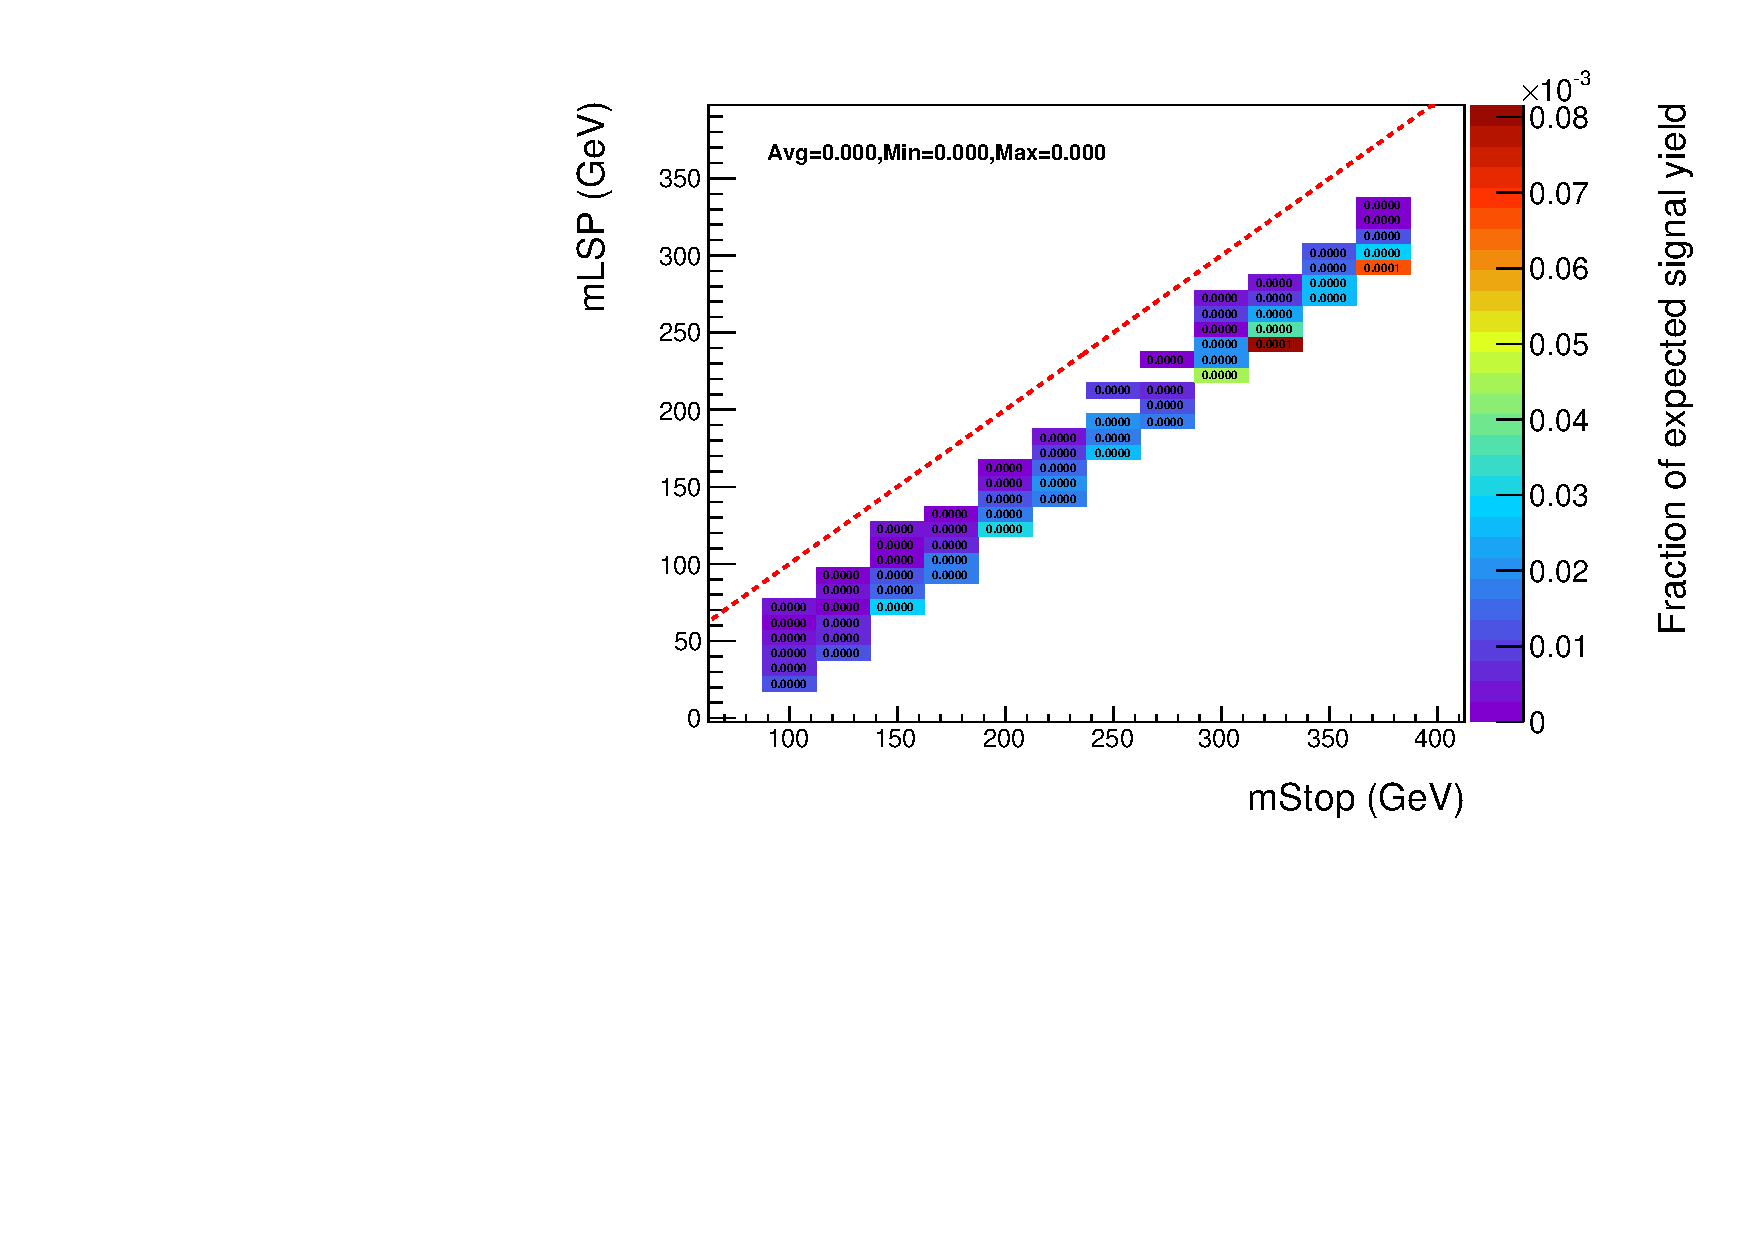
\includegraphics[width=\textwidth]{Figs/sms/t2degen/v23/effs/T2_4body_muon_eff_maps_eq1b_ge4j_SITV.pdf}
    \caption{\mj region, ($\geq 4$,1)}
    \label{fig:t2_4body_mu_eff_ge4j_1b}
  \end{subfigure} \\
  \caption{Signal efficiency times acceptance for the \Ttwodegen simplified, for 
  the hadronic selection (left) and the \mj selection (right), shown for the 
  four most sensitive analysis categories with an inclusive selection on \HT.}
  \label{fig:t2_4body_eff}
\end{figure}

\begin{table}[ht!]
  \caption{Cutflow table for two mass points ($m_{\sTop} = 250$ \gev, $m_
  {\chiz}=240$ \gev and $m_{\sTop} = 250$ \gev, $m_{\chiz}=170$ \gev) of the
  \texttt{T2Degen} signal model.}
  \label{tab:t2_4body_cutflow}
  \centering
  \footnotesize
  \begin{tabular}{ lcc }
    \hline
    \hline
    Cut Name    & \multicolumn{2}{c}{Cumlative Eff. (\%)}\\
    \hline
    ($m_{\sTop}$, $m_{\chiz}$)& (250, 240) & (250, 170) \\
    \hline
    Event Counter & 100.00 & 100.00 \\
    $\nj \geq 2$  & 10.80 & 32.33 \\
    MET Filters & 10.80 & 32.33 \\
    Vertex Noise Filter & 10.80 & 32.33 \\
    HBHE Noise Filter & 10.80 & 32.33 \\
    DeadECAL Filter & 9.13 & 21.30 \\
    $n_{e} = 0$ & 9.13 & 19.70 \\
    $n_{\gamma} = 0$  & 9.13 & 19.55 \\
    $n_{\mu} = 0$ & 9.13 & 17.41 \\
    $\text{EMF}_{max}$ for all jets > 0.1 & 9.13 & 17.41 \\
    Leading jet \Pt > 100 \gev  & 6.01 & 8.70 \\
    Leading jet $\eta$ < 2.5  & 5.70 & 8.37 \\
    Sub-Leading jet \Pt > 100 \gev  & 1.64 & 2.23 \\
    $n_{j, fail} = 0$ & 1.61 & 2.17 \\
    $\Delta R(\mu^i_{fail}, jet^j) < 0.5$ & 1.61 & 2.11 \\
    $(\sum_{}^{n_{vertices}}{\Pt}$) / \HT & 1.61 & 2.11 \\
    recHitCut & 1.61 & 2.11 \\
    $n_{SIT} = 0$ & 1.50 & 1.67 \\
    \mindphistar > 0.3  & 1.35 & 0.93 \\
    \mhtmet < 1.25  & 1.24 & 0.68 \\
    \HT > 375 \gev  & 0.55 & 0.37 \\
    \alphat > 0.55  & 0.26 & VAL \\
    \mhtmet < 1.25  & 0.26 & VAL \\
    \hline
    \hline
  \end{tabular}
\end{table}

\subsubsection{Boost corrections to T2\_4body}
Following generator level studies into the \texttt{T2degen} sample a discrepancy 
between the stop system's boost \Pt with respect to the \texttt{T2cc} sample was
found. As the kinematics of the stop system have no dependence on the 
decay channel, any discrepancy must be artificial and should 
therefore be corrected. A direct comparison between the two samples is
shown in figure~\ref{fig:t2degen_boost_compare}.

\begin{figure}[h!]
  \centering
    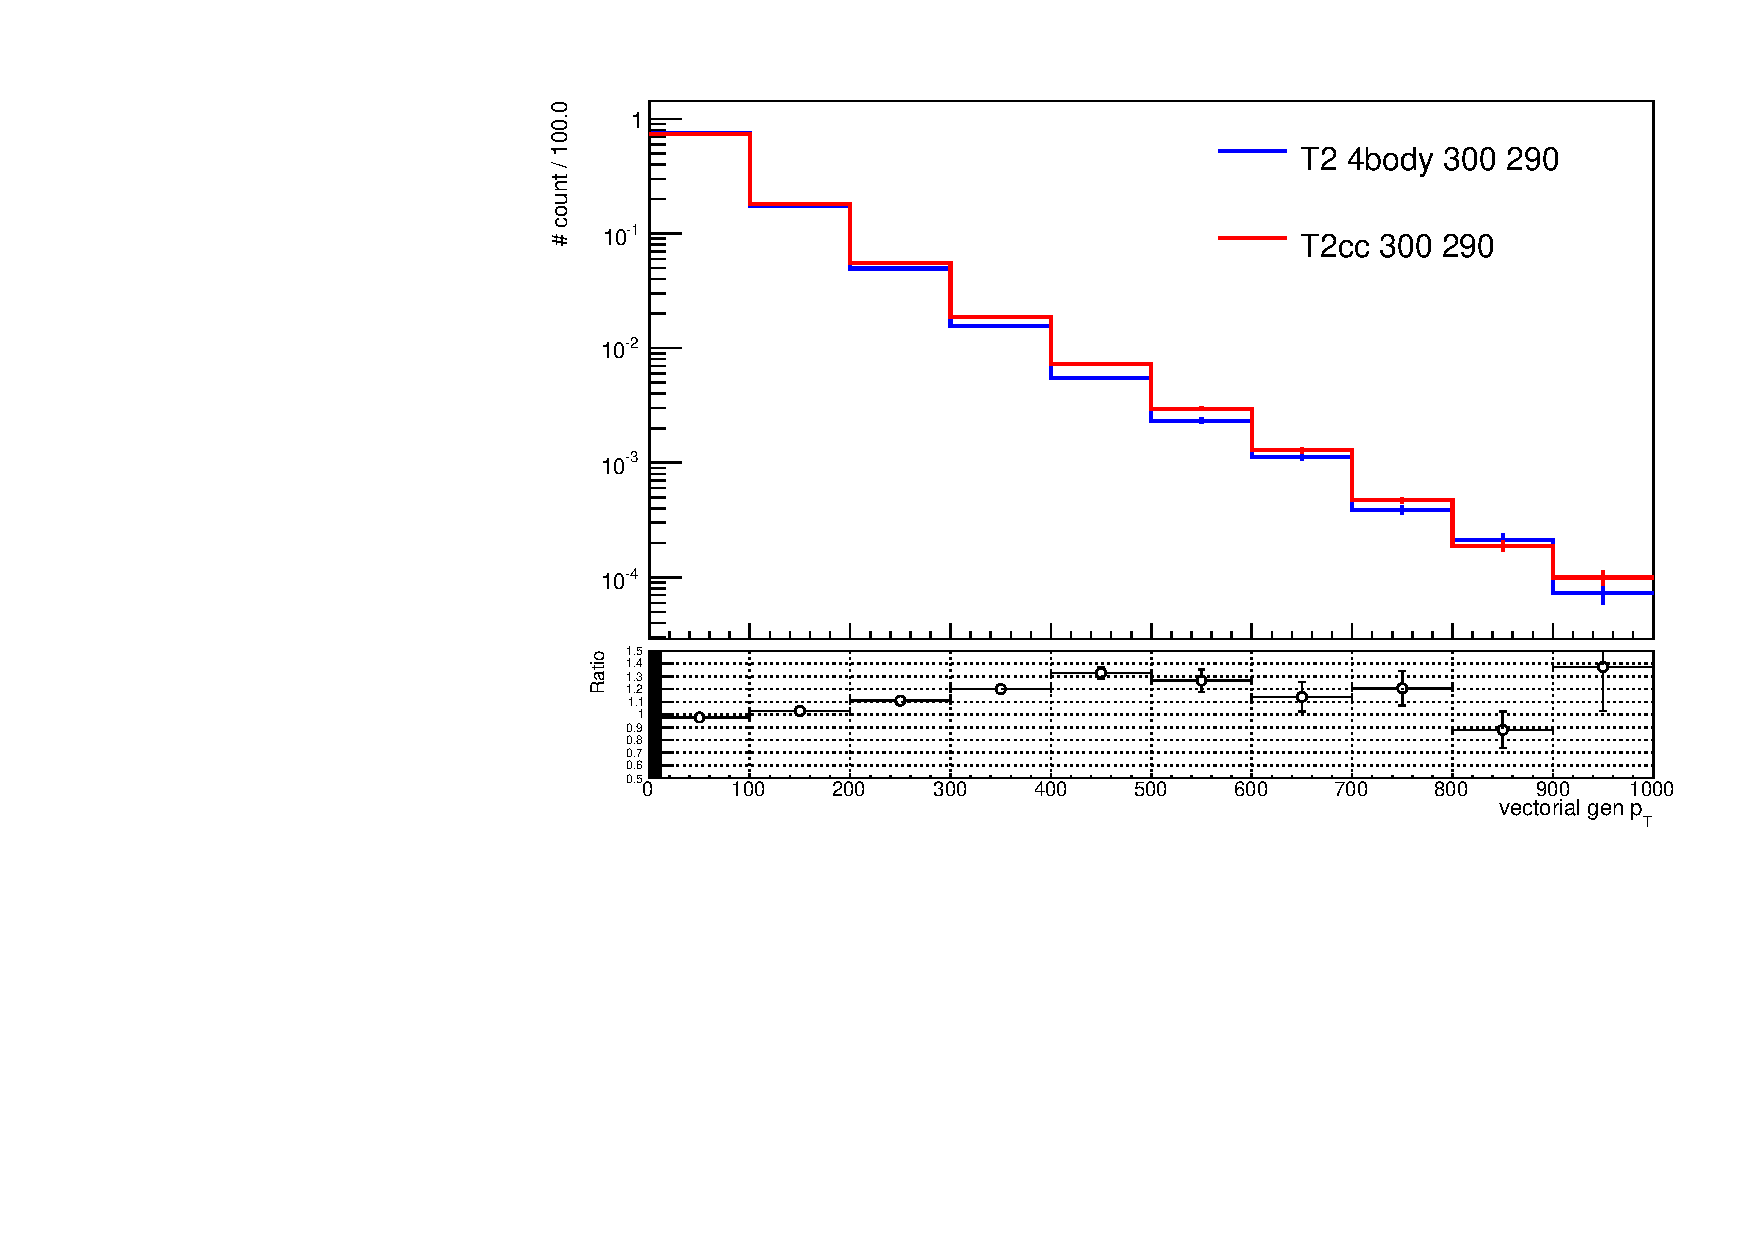
\includegraphics[width=0.6\textwidth]{Figs/sms/t2degen/corrs/compar_stopGenPtVect_0_inc_inc_T2cc_noCuts_sitv_log.pdf}
  \caption{Comparison of the vectorial sum generator-level \Pt of the
  pair-produced \sTop particles, between the \texttt{T2cc} (red) and
  \texttt{T2Degen} (blue) 
  samples, for the mass point (300, 290) \gev. No selection cuts are made and 
  plots are each normalised to a unit area.}
  \label{fig:t2degen_boost_compare}
\end{figure}

% Corrections are taken as the ratio between \texttt{T2Degen} and \texttt{T2cc},
% as a function of the boost \Pt, for each value of $m_{\sTop}$ in the scan. The 
% values of these corrections are shown in figure~\ref{fig:t2degen_boost_weights}.

% \begin{figure}[ht!]
%   \centering
%     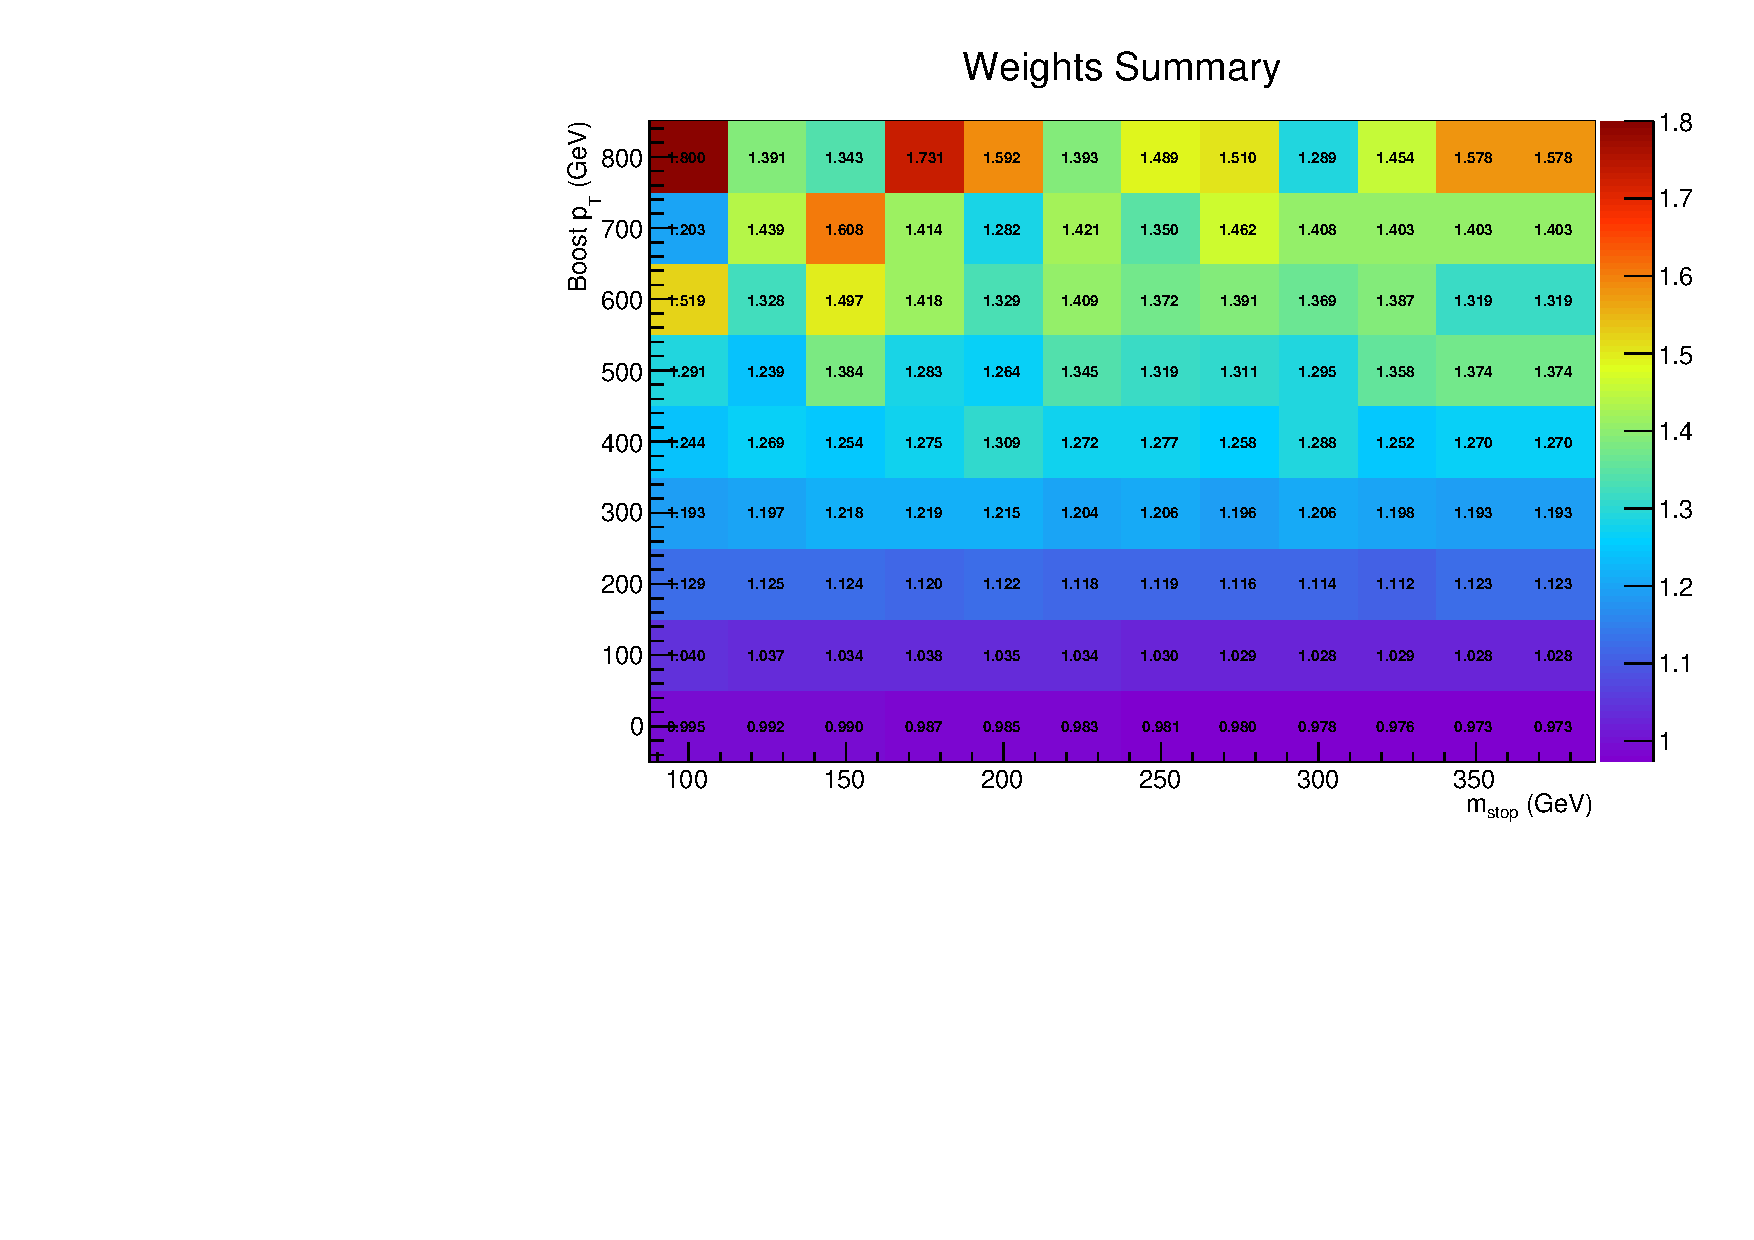
\includegraphics[width=0.8\textwidth]{Figs/sms/t2degen/corrs/stop_lut_weights.pdf}
%   \caption{The weights applied to the \texttt{T2degen} sample, shown as a 
%   function of $m_{\sTop}$ and boost \Pt.}
%   \label{fig:t2degen_boost_weights}
% \end{figure}

% Acceptance at the smallest mass-splittings should be in agreement between 
% both the \texttt{T2cc} and \texttt{T2Degen} samples following these corrections,
% as sensitivity comes entirely from ISR jets and therefore the boost spectrum of 
% the \sTop particles. As shown in \emph{MAKE PLOT SHOWING AGREEMENT}

The discrepancy has been isolated to the 4-body decay model and as a result of
the \Pt distribution of the ISR particles in events with two ISR
particles. By comparison with the charm decay sample, a parameterisation has
been determined as a function of each generator level ISR particle \Pt so
corrective event weights can be calculated REFERENCE TO IVAN ET AL? As a
consequence, this reweighting procedure is applied to the 4-body sample.


\subsection{ISR Corrections to compressed spectra MC signal samples}
\label{sec:isr_reweighting}

Given the reliance of such compressed spectra models on ISR jets for acceptance,
a dedicated study was performed within the SUSY Physics Analysis Group (\emph{PAG})
into the accuracy of it's modelling and relevant systematic uncertainties \cite{susy-isrrw}.

A comparison of data to MC was performed for a pure, high-statistics selection
of Z boson production with associated jets, where the Z decays to an opposite-sign,
same-flavour (OSSF) lepton pair, $Z\ra l\bar{l}$. By tagging the leptons in 
the event, remaining jets can be considered as an ISR jet based ``recoil system'' 
against that of the Z boson decay. Comparisons of data to MC for both the 
vectorial sum of the lepton \Ptvect's and the recoil jet system's \Ptvect indicate an
over-prediction in MC as a function of the system's \Pt, of up to 20\% in 
high \Pt scenarios, shown in figure~\ref{fig:isr_datamc}.

Correction factors for \MADGRAPH based samples, dependent on the \Pt of the jet
system, can therefore be derived by extracting the ratio of data to MC. These 
values are summarised in table~\ref{tab:isr_weights}. Weights are applied to 
both \texttt{T2cc} and \texttt{T2degen} samples at the event level, where the 
event's boost \Pt is determined by calculating the vectorial sum of the 
two, pair-produced generator level \sTop particles.

\begin{table}[ht!]
  \caption{Correction factors for \MADGRAPH based signal samples to account for 
  MC over-prediction of ISR.\label{tab:isr_weights}}
  \centering
  \small
  \begin{tabular}{ lc }
    \hline
    \hline
    $\Pt_{boost}$ (\gev)    & Correction Factor \\
    \hline
    $0 <\Pt\leq120    $          & 1.00 \\
    $120 <\Pt\leq150  $          & 0.95 \\
    $150 <\Pt\leq250  $          & 0.90 \\
    $250 < \Pt        $          & 0.80 \\    
    \hline
    \hline
  \end{tabular}
\end{table}

\begin{figure}[h]
  \begin{center}
    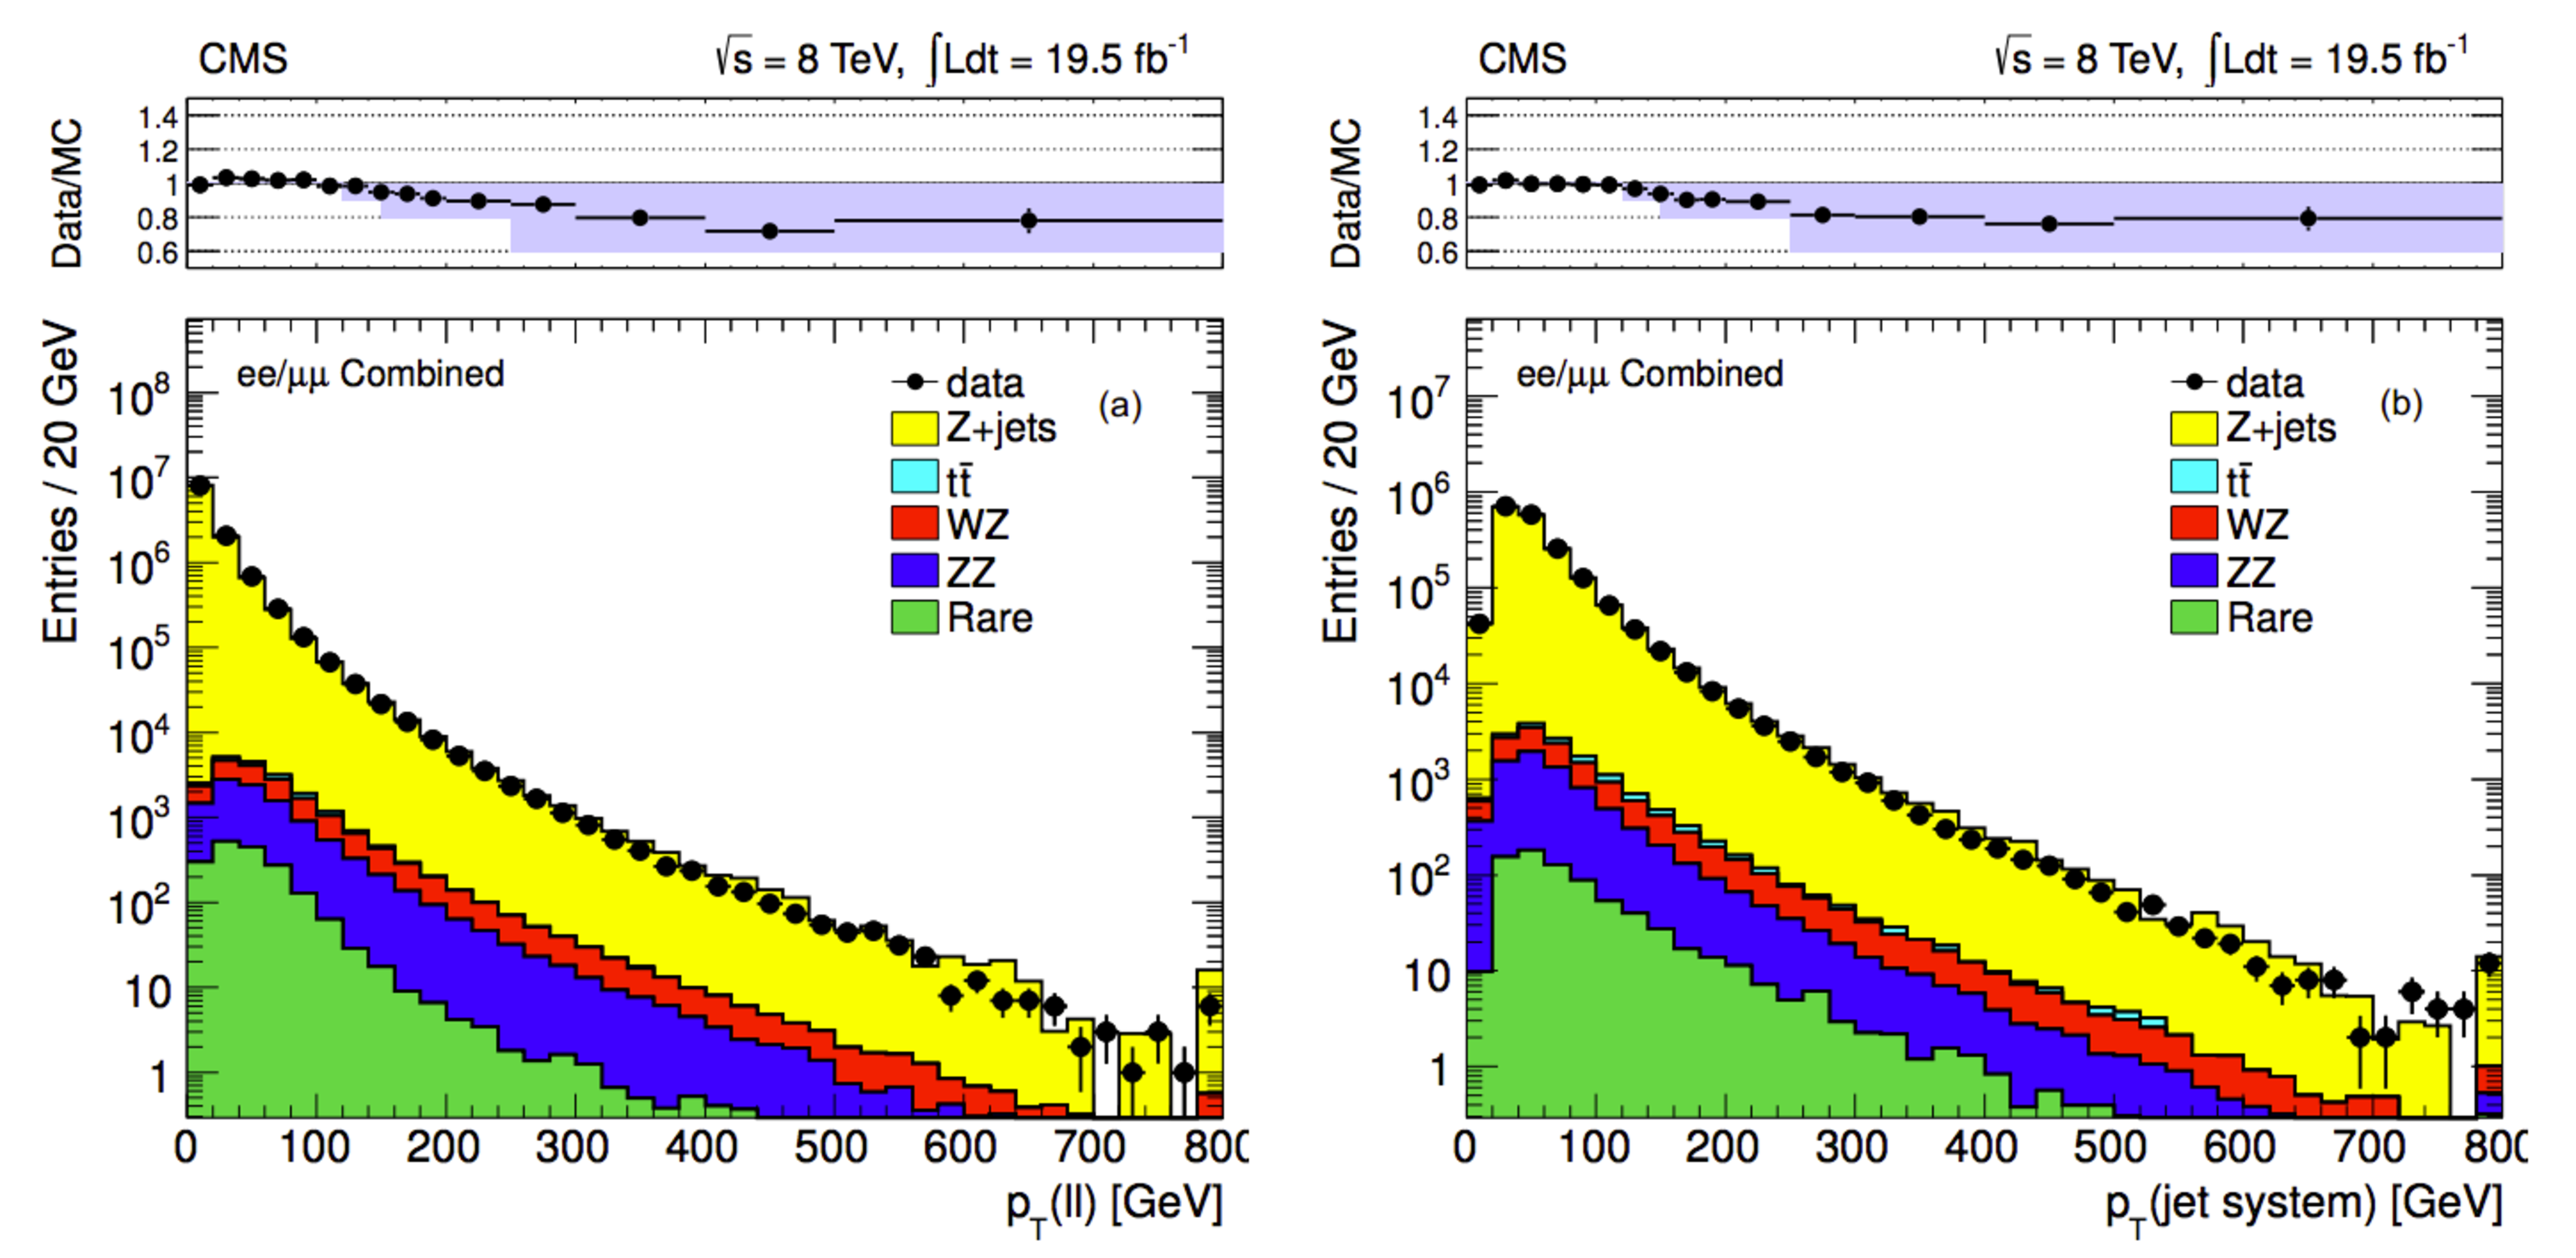
\includegraphics[width=0.8\textwidth]{Figs/isr/isr_zjets_distros.pdf}
    % \caption{blah}
    \caption{Data to MC comparisons for an enriched $Z \ra l\bar{l}$ selection, 
    with the vectorial sum of lepton \Pt's (left) and of the recoil jets (right).
    \cite{susy-isrrw}}
    \label{fig:isr_datamc}
  \end{center}
\end{figure}

\emph{show the effect on signal acceptance for T2cc?}

%********************************** % Second Section  *************************************
\section{Systematic Uncertainties on Signal Acceptance }  %Section - 1.2
\label{sec:interpretation_uncertainties}

A range of sources of systematic uncertainty on the acceptance times signal
efficiency are considered for each signal 
model. The main sources, namely jet energy scale (JES), initial state 
radiation (ISR), b-tag scale factors, parton distribution function (PDF), the 
\mhtmet cut and the dead ECAL filter, have systematic values determined per point
in the scan plane, as a function of \HT, \nb and \nj. The remaining systematics 
are applied as a flat contribution across the entire plane, considered as a 
conservative approach.

Although systematics are considered as a function of the \HT dimension of the 
analysis, all plots shown represent an inclusive selection of \HT>200 \gev.

\subsection{Jet energy scale}
The acceptance times signal efficiency is tested for sensitivity to jet energies by measuring
it's change to upwards and downwards variations of all jet energies by the 
\Pt and $\eta\text{-dependent}$ jet energy scale (JES) uncertainty, as prescribed by 
the JetMET \emph{POG}.

Distributions showing the acceptance changes due to the variations in JES are 
shown in Appendices~\ref{sec:t2cc_jes_plots} for the \texttt{T2cc} model and
\ref{sec:t2degen_jes_plots} for the \texttt{T2Degen} model.

In both models, the effects of applying 
JES variations are stronger in the \njhigh category. An increased number of jets
sharing the small kinematic phase space of the compressed region implies softer jets.
Therefore applying variations on the jet energies increases the probability to move
jets in and out of 
acceptance. This effect is also noticeable in the \njlow, \nb= 1 category for 
\texttt{T2cc} (figure~\ref{fig:sms-jes-t2cc-le3j-1b}), where changes in 
efficiencies are larger away from the diagonal, where acceptance gradually increases
dependence on jets originating from the soft SUSY decay.

The \texttt{T2Degen} model decay contains a real b-quark, and consequently JES 
uncertainties have a dependence on \nb, as higher variations are observed in 
the \nb=1 category (figure~\ref{fig:sms-jes-tdegen-le3j-1b}).


\subsection{Initial State Radiation}
As described in section~\ref{sec:isr_reweighting}, boost \Pt dependent 
event weights are taken from the data to MC comparison study performed within
the SUSY \emph{PAG}. A procedure is also defined to determine related systematics, by
applying upwards and downwards variations of weights corresponding to the 
magnitude of the corrections themselves, and studying the effect on signal 
efficiency times acceptance. These weights are summarised in
table~\ref{tab:isr_syst_weights}.

\begin{table}[ht!]
  \caption{Systematic factors for \MADGRAPH based signal samples to determine 
  ISR modelling related systematics.\label{tab:isr_syst_weights}}
  \centering
  \small
  \begin{tabular}{ lc }
    \hline
    \hline
    $\Pt_{boost}$ (\gev)         & Systematic Variation \\
    \hline
    $0 <\Pt\leq120    $          & $\pm0.0$ \\
    $120 <\Pt\leq150  $          & $\pm0.05$ \\
    $150 <\Pt\leq250  $          & $\pm0.10$ \\
    $250 < \Pt        $          & $\pm0.20$ \\    
    \hline
    \hline
  \end{tabular}
\end{table}

As discussed previously in sections~\ref{sec:t2cc_eff} and \ref{sec:t2degen_eff},
acceptance for compressed spectra models at the smallest \deltam (i.e. nearest 
the diagonal) is predominantly due to presence of hard ISR jets. Away from the
diagonal, ISR jets are still important, instead to boost 
the soft SUSY decay system. Subsequently, systematics due to ISR variations are 
observed to be largest nearest the diagonal for all analysis categories, as shown in
figure~\ref{fig:sms-isr-t2cc} and \ref{fig:sms-isr-t2degen} for \texttt{T2cc} 
and \texttt{T2Degen} respectively. Due to the overall dependence on ISR, the 
related systematics are the largest contribution to the total systematic value.


\subsection{Btag scale factors}
Specifically for \FASTSIM signal samples, events are not weighted using the 
b-tag formula method described in section~\ref{sec:formula_method}, but instead
using the 
recommended method for \FULLSIM samples with an additional \FULLSIM to \FASTSIM 
correction factor applied. The original correction is dependent on the generator
level content of an event, and is defined as:
% 
\begin{equation}
w = \frac{SF_b \epsilon \times (1-SF_b \epsilon) \times SF_{c,light} m \times (1
-SF_{c,light} m)}{\epsilon \times (1-\epsilon) \times m \times (1-m)}
\label{eq:btag_fullsim_weight}
\end{equation}
% 
where $\epsilon(\Pt, \eta)$ and $m(\Pt, \eta)$ are the b-tagging efficiency and 
mistagging rate, respectively. These factors are functions of \Pt and $\eta$, and
are measured in SM MC for both the hadronic and \mj samples, in each \HT bin.

Applying this event weight provides `corrected' MC yields, which then 
have further \FASTSIM to \FULLSIM correction factors applied, as recommended by
\cite{btagpogtwiki}.

Systematic variations equal to the errors of these corrections are applied as 
upwards and downwards variations, and any effects on signal efficiency times 
acceptance are studied.

As expected, only small changes in acceptance are found in the \texttt{T2cc} 
model when b-tag scale factor variations are applied, as shown in
figure~\ref{fig:sms-btag-t2cc}. While not entirely negligible, it is worth 
noting that systematics are slightly larger for the \nb= 1 category
(figure~\ref{fig:sms-btag-t2cc-le3j-1b}), however still at a low level with 
respect to other systematic sources.

% The \texttt{T2Degen} model, containing a real b-quark, has WHAT?
% \emph{Why is T2degen at the same level as T2cc? Is that correct??}
The \texttt{T2Degen} model exhibits a similar dependence on the b-tag scale
factor variations, indicating large changes in efficiency nearer the diagonal in
\nb = 1 categories. This increase is visible in
figure~\ref{fig:sms-btag-t2degen-le3j-1b} at smaller values of \deltam, where
the final state b-quark is likely out of acceptance, and therefore tags
originate from mis-tagged lighter quarks or gluons.


\subsection{PDF}
Montecarlo generation includes a simulation of the Parton Density Function (PDF) 
of the incoming partons, described by a `PDF set'. Signal samples are produced
using the \textsc{CTEQ6L1} PDF set. The acceptance 
sensitivity to the PDF set is investigated by comparing results using three
other commonly used PDF sets, namely \textsc{CT10}, \textsc{NNPDF2.1} and
\textsc{MSTW2008}. Following PDF4LHC recommendations, the output is 
combined to determine an `envelope' value combining the three alternative PDF 
sets, and a related systematic uncertainty \cite{pdf4lhc}.

The effect on selection efficiency was studied for \texttt{T2cc} with the
central value and upwards and downwards fluctuation plots summarised in
figure~\ref{fig:sms-pdf-t2cc}. The largest variations are taken as the
systematic uncertainty for both the \texttt{T2cc} and \texttt{T2Degen} models,
given their identical initial states.

\subsection{\mhtmet cleaning cut}
\label{sec:mhtmet_syst}
The efficiency of the \mhtmet cleaning cut is compared between data and MC with 
the aim of revealing any potential issues due to MC mis-modelling of the 
variable. Efficiencies are compared in the \mj control sample, using \HT bins 
ranging from $200 < \HT < 375$ \gev, in both \nj categories, with no requirement
on \nb. Efficiencies are summarised in table~\ref{tab:mht-met}, where 
efficiency comparisons between data and MC are shown to statistically agree
with unity.

% \emph{this covers \FULLSIM and data agreement, but what do we do for \FASTSIM to 
% \FULLSIM agreement?}

\begin{table}[!h]
  \caption{Efficiencies of the \mhtmet requirement cut for the \mj selection in
  data
  $\epsilon_{\text{data}}$ and MC $\epsilon_{\text{MC}}$, as well as the ratio
  of both. Efficiencies are shown for the two \nj categories and the four lowest
  \HT bins, with an inclusive requirements are made of \nb.
  }
  \label{tab:mht-met}
  \centering
  \footnotesize
  \begin{tabular}{ ccccc }
    \hline
    \hline
    \nj    & \HT (GeV) & $\epsilon_{\text{MC}}$ & $\epsilon_{\text{data}}$ & $\epsilon_{\text{MC}}/\epsilon_{\text{data}}$ \\
    \hline
    2--3     & 200--275      & $0.95 \pm 0.00$        & $0.95 \pm 0.01$          & $1.00 \pm 0.01$                               \\
    2--3     & 275--325      & $0.97 \pm 0.01$        & $0.97 \pm 0.02$          & $1.00 \pm 0.02$                               \\
    2--3     & 325--375      & $0.97 \pm 0.01$        & $0.97 \pm 0.02$          & $1.00 \pm 0.02$                               \\
    2--3     & 375--475      & $0.98 \pm 0.01$        & $0.98 \pm 0.03$          & $1.00 \pm 0.03$                               \\
    $\geq 4$ & 200--275      & $0.90 \pm 0.02$        & $0.92 \pm 0.04$          & $0.98 \pm 0.04$                               \\
    $\geq 4$ & 275--325      & $0.92 \pm 0.01$        & $0.93 \pm 0.02$          & $0.99 \pm 0.02$                               \\
    $\geq 4$ & 325--375      & $0.92 \pm 0.01$        & $0.93 \pm 0.04$          & $0.99 \pm 0.04$                               \\
    $\geq 4$ & 375--475      & $0.95 \pm 0.02$        & $0.95 \pm 0.04$          & $1.00 \pm 0.04$                               \\
    \hline
    \hline
  \end{tabular}
\end{table}

While the relevant systematic for the \mhtmet requirement is taken from the
above method, it is also interesting to study the acceptance of this cut as a
function of the mass plane for each decay.
Model acceptance to the \mhtmet cut is typically lower in the 4-body decay. This
is attributed to the softer jet spectrum produced due to the increased number of
final state particles sharing the finite energy of the decay system.

\subsection{Dead ECAL Filter}
To assess any potential MC mis-modelling issues with the dead ECAL filter, a 
similar analysis is made as described for the \mhtmet cut in
section~\ref{sec:mhtmet_syst}. 
Efficiencies between data and MC are compared for the \mj selection, with an 
inclusive requirement on both \nb and \HT. As shown in table~\ref{tab:dead-ecal},
the ratio of efficiencies between data and MC for each \nj category agree within
statistical errors.

% \emph{\FULLSIM to \FASTSIM systs?}

\begin{table}[!h]
  \caption{Efficiencies of the dead ECAL cut for the \mj selection in data
  $\epsilon_{\text{data}}$ and MC $\epsilon_{\text{MC}}$, as well as the ratio
  of both. Efficiencies are shown for the two \nj categories and the four lowest
  \HT bins, with an inclusive requirements are made of \nb.}
  \label{tab:dead-ecal}
  \centering
  \footnotesize
  \begin{tabular}{ ccccc }
  % \begin{tabular}{ ccc }
    \hline
    \hline
    \nj    & \HT (GeV) & $\epsilon_{\text{MC}}$ & $\epsilon_{\text{data}}$ & $\epsilon_{\text{MC}}/\epsilon_{\text{data}}$ \\
    % \nj     & \HT (GeV) & $\epsilon_{\text{MC}}/\epsilon_{\text{data}}$                                                     \\
    \hline
    2--3     & $>200$        & $0.64 \pm 0.01$        & $0.64 \pm 0.01$          & $1.00 \pm 0.01$                               \\
    $\geq 4$ & $>200$        & $0.58 \pm 0.01$        & $0.59 \pm 0.01$          & $0.98 \pm 0.01$                               \\
    % 2--3      & $>200$        & $1.00 \pm 0.01$                                                                                   \\
    % $\geq 4$  & $>200$        & $0.98 \pm 0.01$                                                                                   \\
    \hline
    \hline
  \end{tabular}
\end{table}

Similarly to the study of the \mhtmet requirement, an inspection of the
acceptance of the dead ECAL filter in each scan plane indicates a greater
reduction in acceptance for the 4-body decay
with respect to the charm decay. The larger number of particles in the final
state of the 4-body decay increases the probability for an energy deposit to be
made near a flagged region of the calorimeter system, thereby rejecting more
events. Rejection increases away from the diagonal, as more objects move into
acceptance.

\emph{but the \nj requirements are the same between samples...perhaps the
fraction of 3jet/2jet within the le3j category, is greater for 4body?}

\subsection{Generator Level Partons}
At the \MADGRAPH matrix element stage of the MC simulation production, a number
of additional feynman diagrams are simulated to account for associated parton 
interactions, such as Initial State Radiation (ISR) and Final State Radiation
(FSR). Given the dependence on such processes in the
compressed spectra regime, an additional sub-sample of the \texttt{T2cc} scan 
has been produced with up to 3 additional partons, to compare against the up to
2 additional partons of the complete scan. This sample contains two mass points 
at a stop mass near the region of maximum sensitivity, with mass splittings 
covering both extremeties of the scan ($\deltam = 10$ \gev, 80 \gev). The relative
change in efficiency times 
acceptance between the two scans is shown in table~\ref{tab:sms-t2cc-2v3part}. 
These values are interpretted as systematic uncertainties on the number of 
associated partons modelled for such compressed spectra models, and are applied 
as flat contributions across the scan plan for all models.

\begin{table}[!h]
  \caption{Relative change in efficiency times acceptance for the
    2-parton and 3-parton scans in the signal region, with an inclusive 
    selection on \nb and \HT>200 \gev. The scan points are $m_{\sTop} = 200$ \gev 
    and $m_{\chiz} = (120, 190)$ \gev.}
  \label{tab:sms-t2cc-2v3part}
  \centering
  \small
  \begin{tabular}{ lcc }
    \hline
    \hline
    Category     & \multicolumn{2}{c}{$\Delta m$ (GeV)} \\
    \cline{2-3}
                 & 10   & 80                            \\
    \hline
    (2--3,0)     & 0.00 & 0.04                          \\
    (2--3,1)     & 0.02 & 0.04                          \\
    ($\geq 4$,0) & 0.04 & 0.04                          \\
    ($\geq 4$,1) & 0.00 & 0.00                          \\
    \hline
    \hline
  \end{tabular}
\end{table}

\subsection{Luminosity Measurement}
Flat corrections across the scan plane are made to account for the uncertainty 
of the luminosity measurement, as quoted by Lumi \emph{POG} at 2.5\%
\cite{CMS:2013gfa}.

\subsection{Summary}

For each mass point in the scan plane, the total systematic is the sum in 
quadrature of all individual contributions. Representative values are summarised
in tables~\ref{tab:sms-syst-t2cc} and \ref{tab:sms-syst-t2_4body}, with full
results shown in figures~\ref{fig:sms-totalsyst-t2cc} and
\ref{fig:sms-totalsyst-t2degen} in the mass plane of \texttt{T2cc} and
\texttt{T2Degen} respecitively. The distribution of total systematic values seen
in these plots has been corrected to account for statistical fluctations through
the use of an iterative smoothing procedure that considers a weighted average of
each mass point value of the surrounding points. This procedure is carefully
checked to ensure no loss of total systematic trends in either $m_{\sTop}$ or
\deltam.

\begin{table}[h!]
  \caption{Representative ranges for each contribution to the total
    systematic uncertainty on the signal efficiency times acceptance
    for each relevant event category for the \texttt{T2cc}
    interpretation. 
    \label{tab:sms-syst-t2cc}
  }   
  \centering
  \small
  \begin{tabular}{ lcccccccccc }
    \hline
    \hline
    Category   & \multicolumn{2}{c}{(2--3,0)} & \multicolumn{2}{c}{(2--3,1)}     &\multicolumn{2}{c}{($\geq 4$,0)} & \multicolumn{2}{c}{($\geq 4$,1)} & \multicolumn{2}{c}{($\geq 2$,$\geq 0$)} \\
    Range      & Min.      & Max.             & Min.     & Max.                  & Min.    & Max.                  & Min.    & Max.        & Min.    & Max.  \\
    \hline
    PDF        &           &                  &          &                       &         &                       &         &             & 0.04    & 0.14  \\
    JES        & 0.01      & 0.12             & 0.01     & 0.18                  & 0.10    & 0.23                  & 0.07    & 0.23        && \\
    ISR        & 0.09      & 0.21             & 0.08     & 0.21                  & 0.13    & 0.22                  & 0.13    & 0.23        && \\
    b-tag SF   & 0.01      & 0.02             & 0.03     & 0.07                  & 0.01    & 0.02                  & 0.02    & 0.07        && \\
    \mht/\met  & 0.02      & 0.02             & 0.02     & 0.02                  & 0.02    & 0.02                  & 0.02    & 0.02        && \\
    Dead ECAL  & 0.02      & 0.02             & 0.02     & 0.02                  & 0.02    & 0.02                  & 0.02    & 0.02        && \\
    \hline
    Total syst & 0.14      & 0.21             & 0.16     & 0.22                  & 0.22    & 0.26                  & 0.23    & 0.30        && \\
    \hline
    \hline
  \end{tabular}
\end{table}

\begin{table}[h!]
  \caption{Representative ranges for each contribution to the total
    systematic uncertainty on the signal efficiency times acceptance
    for each relevant event category for the \texttt{T2Degen}
    interpretation.  
    \label{tab:sms-syst-t2_4body}
  }   
  \centering
  \small
  \begin{tabular}{ lcccccccccc }
    \hline
    \hline
    Category   & \multicolumn{2}{c}{(2--3,0)} & \multicolumn{2}{c}{(2--3,1)}     &\multicolumn{2}{c}{($\geq 4$,0)} & \multicolumn{2}{c}{($\geq 4$,1)} & \multicolumn{2}{c}{($\geq 2$,$\geq 0$)} \\ 
    Range      & Min.      & Max.             & Min.     & Max.                  & Min.    & Max.                  & Min.    & Max.                   & Min.      & Max.\\
    \hline                                                                                                                                              
    PDF        &           &                  &          &                       &         &                       &         &                        & 0.04      & 0.14\\
    JES        & 0.00      & 0.12             & 0.00     & 0.19                  & 0.01    & 0.32                  & 0.02    & 0.40                   &           &\\
    ISR        & 0.07      & 0.20             & 0.05     & 0.21                  & 0.10    & 0.22                  & 0.06    & 0.22                   &           &\\
    b-tag SF   & 0.01      & 0.02             & 0.01     & 0.07                  & 0.01    & 0.04                  & 0.00    & 0.07                   &           &\\
    \mht/\met  & 0.02      & 0.02             & 0.02     & 0.02                  & 0.02    & 0.02                  & 0.02    &  0.02                  &           &\\
    Dead ECAL  & 0.02      & 0.02             & 0.02     & 0.02                  & 0.02    & 0.02                  & 0.02    &  0.02                  &           &\\
    \hline                                                                                                                                                        
    Total syst & 0.18      & 0.21             & 0.21     & 0.23                  & 0.25    & 0.31                  & 0.27    & 0.45                   &           &\\
    \hline
    \hline
  \end{tabular}
\end{table}

%********************************** % Third Section  *************************************
\section{Limits on models of Supersymmetry}  %Section - 1.3
\label{sec:interpretation_limits}

\subsection{Overview of limit setting procedure}
Signal models are tested for compatibility with observations using
a modified frequentist method, namely `CLs' \cite{alread-cls}. A test statistic,
used to rank
experiments from least to most signal-like, is defined as:
% 
\begin{equation}
q_{\mu} = \begin{cases} -2log\lambda(\mu), & \mbox{if } \mu \geq \hat{\mu} \\
0., & \mbox{otherwise} \end{cases},
\end{equation}
% 
where:
% 
\begin{equation}
\lambda(\mu) = \frac{L(\mu, \theta_{\mu})}{L(\hat{\mu}, \hat{\theta_{\mu}})},
\end{equation}
% 
$\mu$ is the signal strength parameter (equivalent to the variable $f$ defined
in section~\ref{sec:results_likelihood}, where $\mu=1$ represents a given
signal at it's nominal cross-section), $\theta_{\mu}$ is a set of nuisance 
parameters for a given $\mu$, $\hat {\mu}$ is the Maximum Likelihood
(ML) value of $\mu$, and $\hat{\theta}$ is the corresponding ML set of nuisance
parameters.

Distributions of $q_{\mu}$ are populated from pseudo-experiments under
signal+background and background only hypotheses. For a given observation, 1
minus the quantiles of each distribution are used to determine $CL_{s+b}$ and
$CL_b$, which are used to define:
% 
\begin{equation}
CL_s = \frac{CL_{s+b}}{CL_b}.
\end{equation}
% 
A model is considered to be excluded at 95\% confidence level if
$CL_s \leq 0.05$.

\emph{maybe include razor example distribution from SUS12005}

\subsection{Limits}
Limits are calculated using 1000 pseudo-experiments per model mass point.
Expected limits are determined by considering a scenario where data observations
are assumed to be equal to the result of the green-band fits
(section~\ref{sec:results_fit_green}), and observed
limits by considering that actual data observations.
A point is considered excluded if the calculated upper limit cross section is
less than the nominal cross-section (NLO+NLL).

\begin{figure}[h!]
\centering
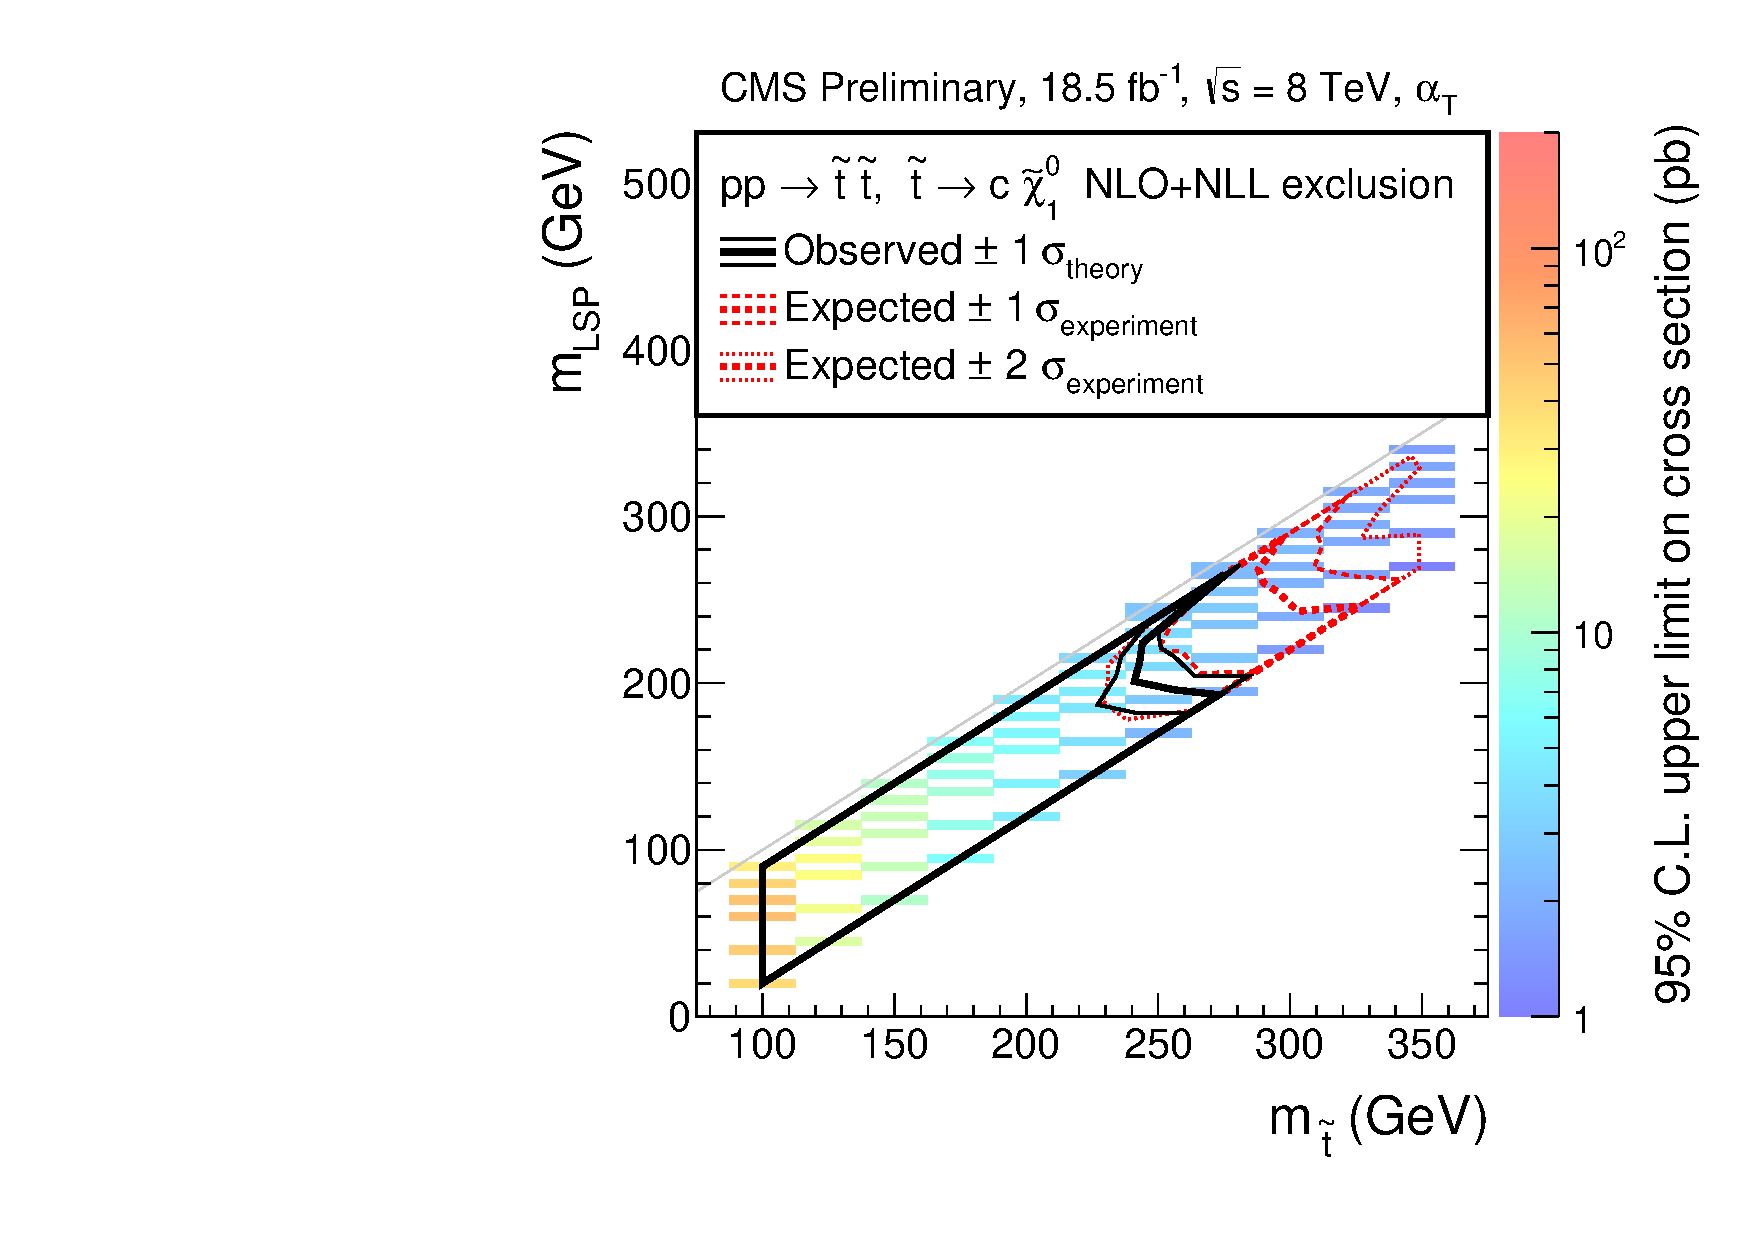
\includegraphics[width=0.85\textwidth]{Figs/sms/t2cc/limit_v0/T2cc_toys_XSEC.pdf}
\caption{The expected limit (red dashed line) with central band (thick red)
and $\pm1\sigma$ and $\pm2\sigma$ uncertainty bands (thin red), and the
observed limit (thick black) for the \texttt{T2cc} model. The limit is
calculated with an include \HT>200 \gev selection, and the analysis categories 
($\nb = 0, \njlow$), ($\nb = 1, \njlow$), ($\nb = 0, \njhigh$), ($\nb = 1,
\njhigh$)}
\label {fig:t2cc_limit}
\end{figure}

\begin{figure}[h!]
\centering
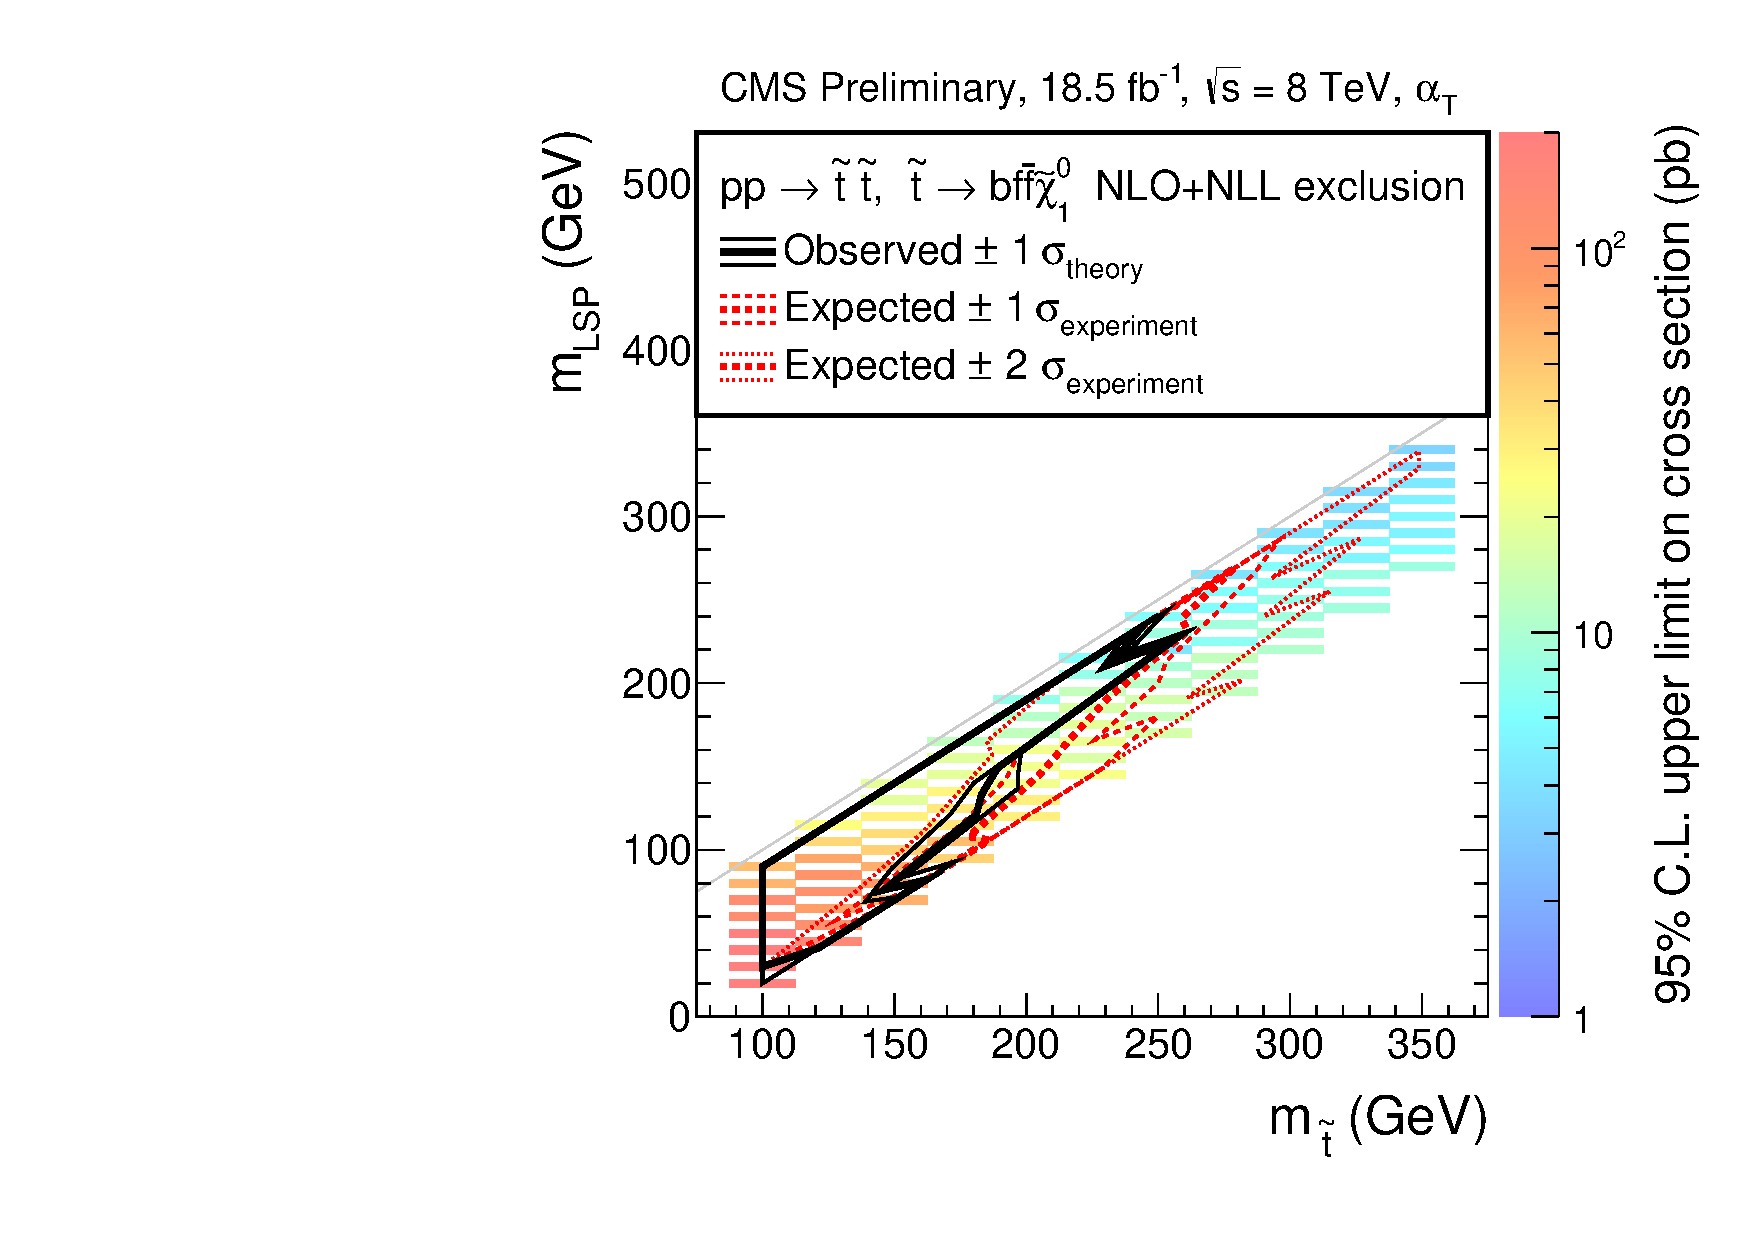
\includegraphics[width=0.85\textwidth]{Figs/sms/t2degen/limit_v0/T2degen_toys_XSEC.pdf}
\caption{The expected limit (red dashed line) with central band (thick red)
and $\pm1\sigma$ and $\pm2\sigma$ uncertainty bands (thin red), and the
observed limit (thick black) for the \texttt{T2degen} model. The limit is
calculated with an include \HT>200 \gev selection, and the analysis categories 
($\nb = 0, \njlow$), ($\nb = 1, \njlow$), ($\nb = 0, \njhigh$), ($\nb = 1,
\njhigh$)}
\label{fig:t2degen_limit}
\end{figure}

%********************************** % Fourth Section  *************************************
\section{Interpretation of excesses}
\label{sec:interpretation_excess}
best fit points in T2cc